\part{设计分析}

\section{信道编码}

某数据传输系统,试图利用300-3400Hz的话音通道进行载波传输,波形信道为加性高斯白噪声信道。采用线性传输,收发两端拟采用滚降系数0.5的根号升余弦滤波,以解决采样点失真问题。数据文件大小为1kB,希望在5秒钟之内传完,即信道中传输的波形时间长度不超过5秒。
    
\subsection{任务分析}

已知话音通道的频带范围为300$\sim$3400Hz,对应的基带带宽为
\begin{equation*}
W=\frac{f_H-f_L}{2}=1550Hz
\end{equation*}

由于采用根号升余弦滤波,可以推导得符号率
\begin{equation*}
R_s=\frac{1}{T_s}\leq\frac{2W}{1+\alpha}=2067\text{Baud}
\end{equation*}

不妨取$R_s$=2000Buad,则在5秒钟的通信时间中可以传输10000个符号。待传输的数据总量为1KByte=8Kbit,因此在无编码的情况下,只能采用二进制的映射方式。不妨采取BPSK的映射方式,即双极性二元码。

以上讨论只是针对无信道编码的情况。信道编码可以通过不同的方式增加或减少信息的冗余,这样就可以利用四进制或八进制的映射方式,这些情况会在之后的部分加以讨论。

\subsection{发射机实现}

根据题目要求,整体通信系统采用滚降系数为0.5的升余弦滚降设计,满足奈奎斯特第一准则,可以找到满足码间无串扰的采样点。MATLAB中自带的rcosdeign()函数即可给出滤波器精确到若干个时域符号,每个符号有若干个的采样值的时域参数,与自己实现的基本一致。下图所示为滤波器的时域和频域波形。

\begin{figure}[h]
    \centering
    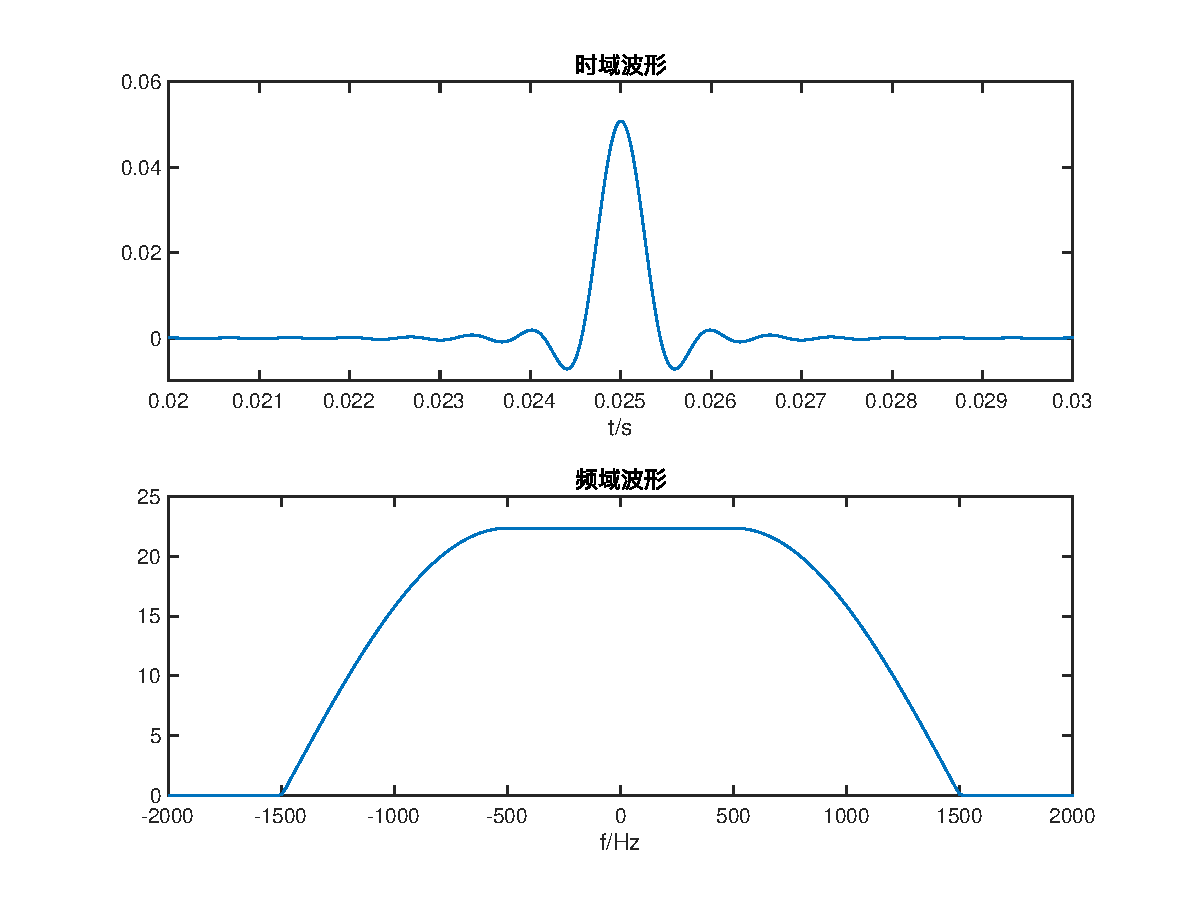
\includegraphics[width=0.5\textwidth]{./pic/rcos_fir.eps}
    \caption{根升余弦棍将滤波器的时域和频域响应}
\end{figure}

载波调制则是直接将基带波形与正弦波在时域相乘,在频域上即可等效为将基带波形成搬移到对应的频带上。对于复电平,应生成频率相同但相位相差$\frac{\pi}{2}$的同频正弦波分别作为I路和Q路的载波,两路之间彼此正交。符号率$R_s$=2000Baud,载波的中心频率为1850Hz。

\subsection{接收机实现}

收端进行解调时,采用相干解调的方法,将对应相位的正弦波与接收到的波形相乘,即可得到对应分量。解调至基带后,通过匹配滤波器对波形进行滤波,得到的波形可以找到满足码间无串扰的采样点。由于根升余弦滤波器本身具有低通特性,相干解调产生的高频分量可以被自动滤除。由于各符号对应的波形相同,信息全部由波形的幅度携带,因此可以只用一路匹配滤波器,然后对最佳采样点的采样值的幅度进行判决。这样的设计可以降低接收机的复杂度。

假设接收机可以完美地恢复出信号的时钟分量。下图分别为发射机中脉冲成型后的基带波形和上变频后的载波形、接收机接收到的载波波形和经过相干解调的基带波形,以及它们各自的功率谱,此时信噪比为10dB。

\begin{figure}[h]
    \centering
    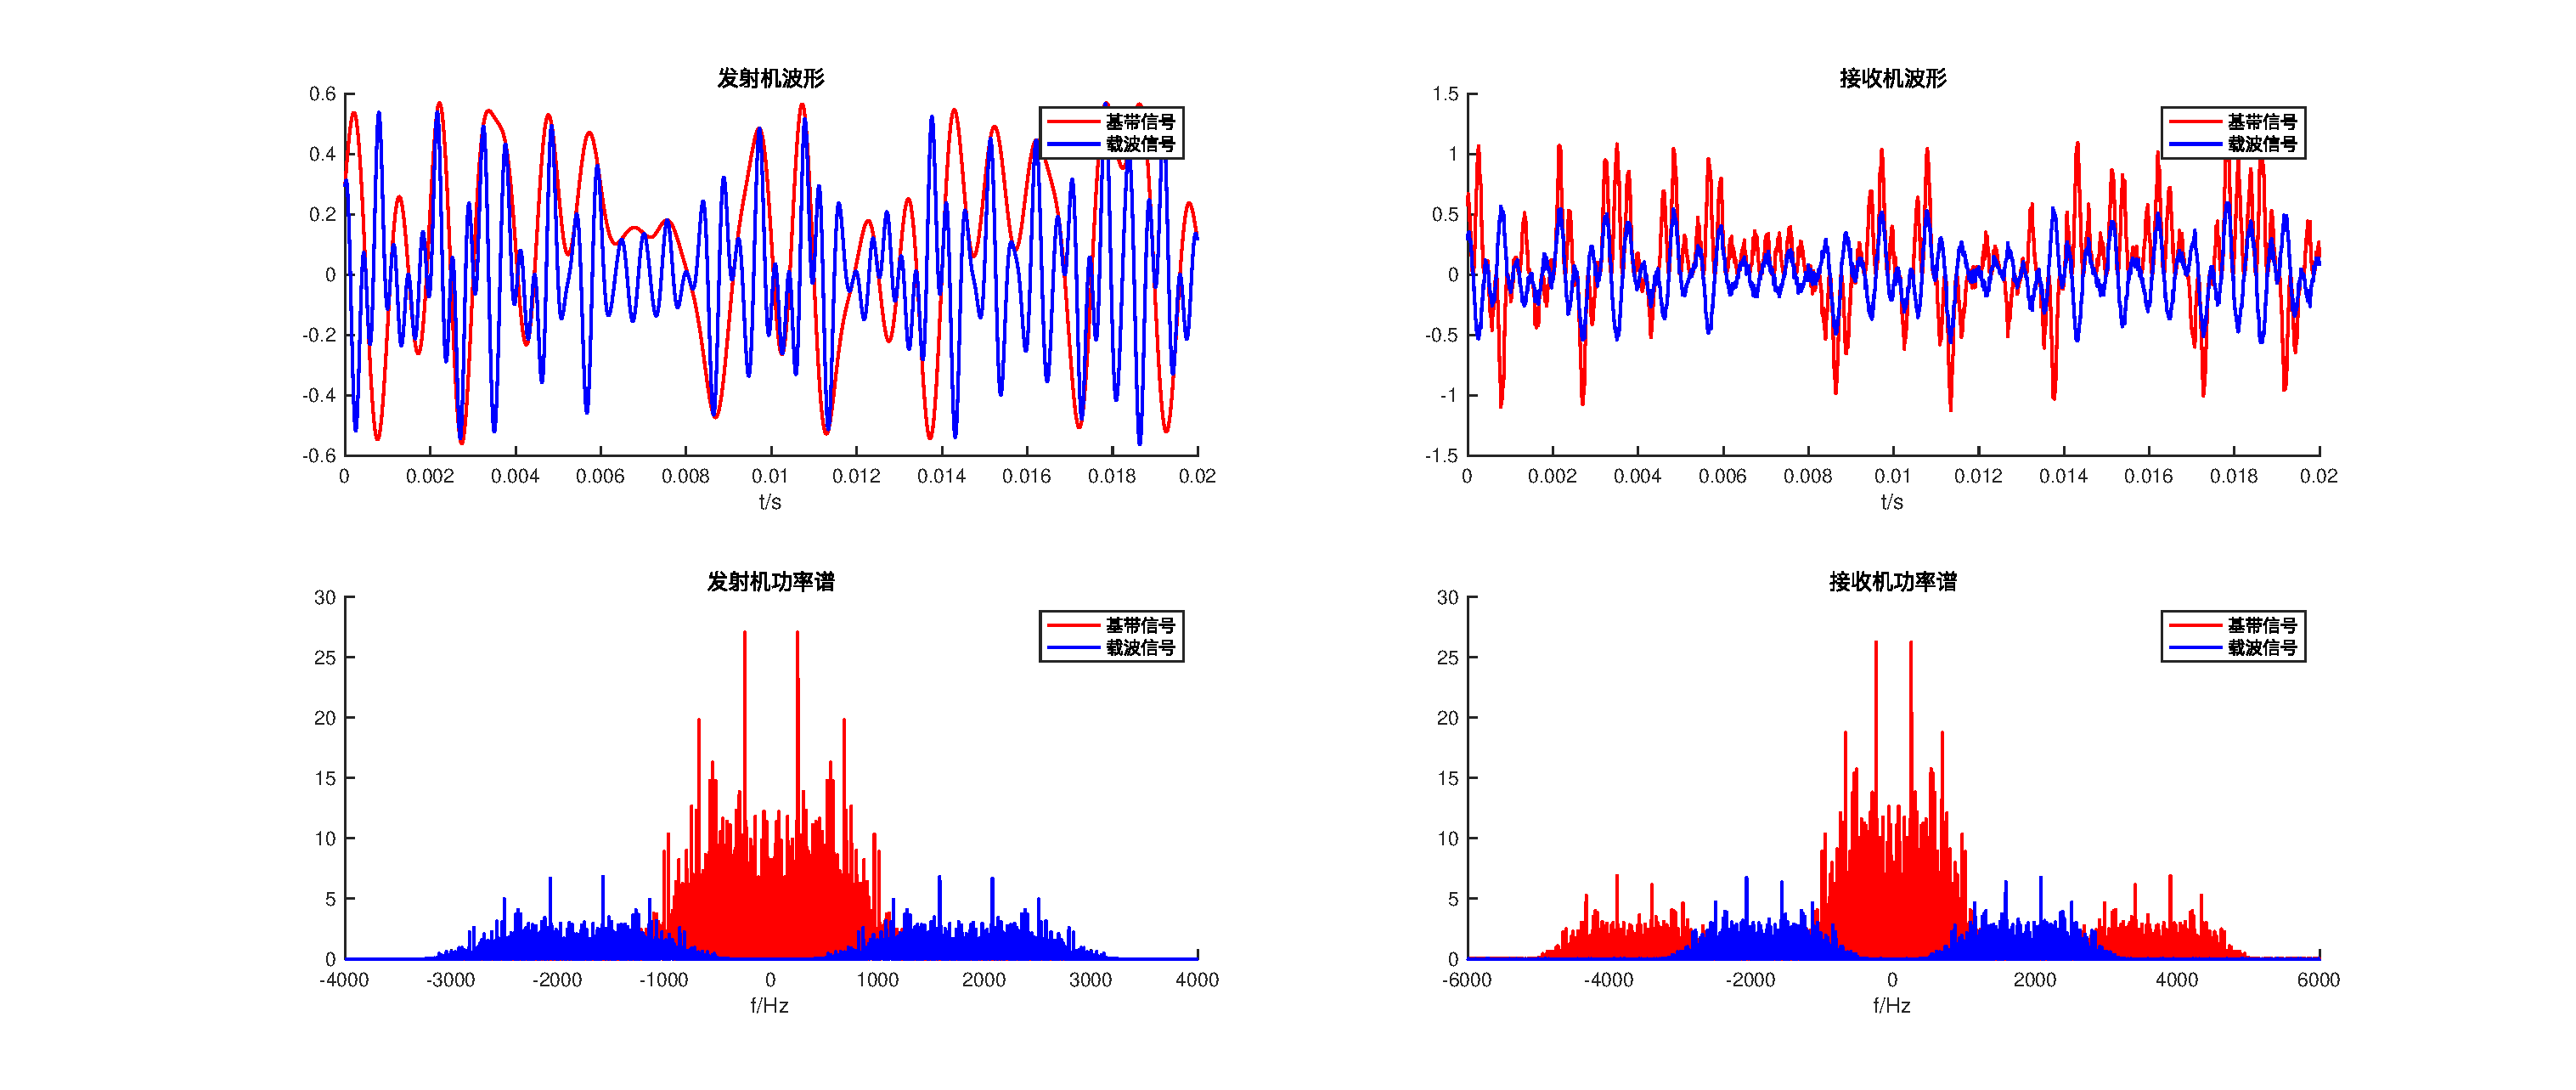
\includegraphics[width=\textwidth]{./pic/wave_spectrum.eps}
    \caption{发射机和接收机的波形与功率谱}
\end{figure}

可以看到由于加性高斯白噪声的影响,功率谱似乎整体多了一个直流分量。波形也出现了许多毛刺。相干解调则把高频的峰向更高频带搬移。具体的采样结果如下图所示,可以看到最佳采样点处得到的结果与原电平非常接近,可以作为之后判决的判据。

\begin{figure}[h]
    \centering
    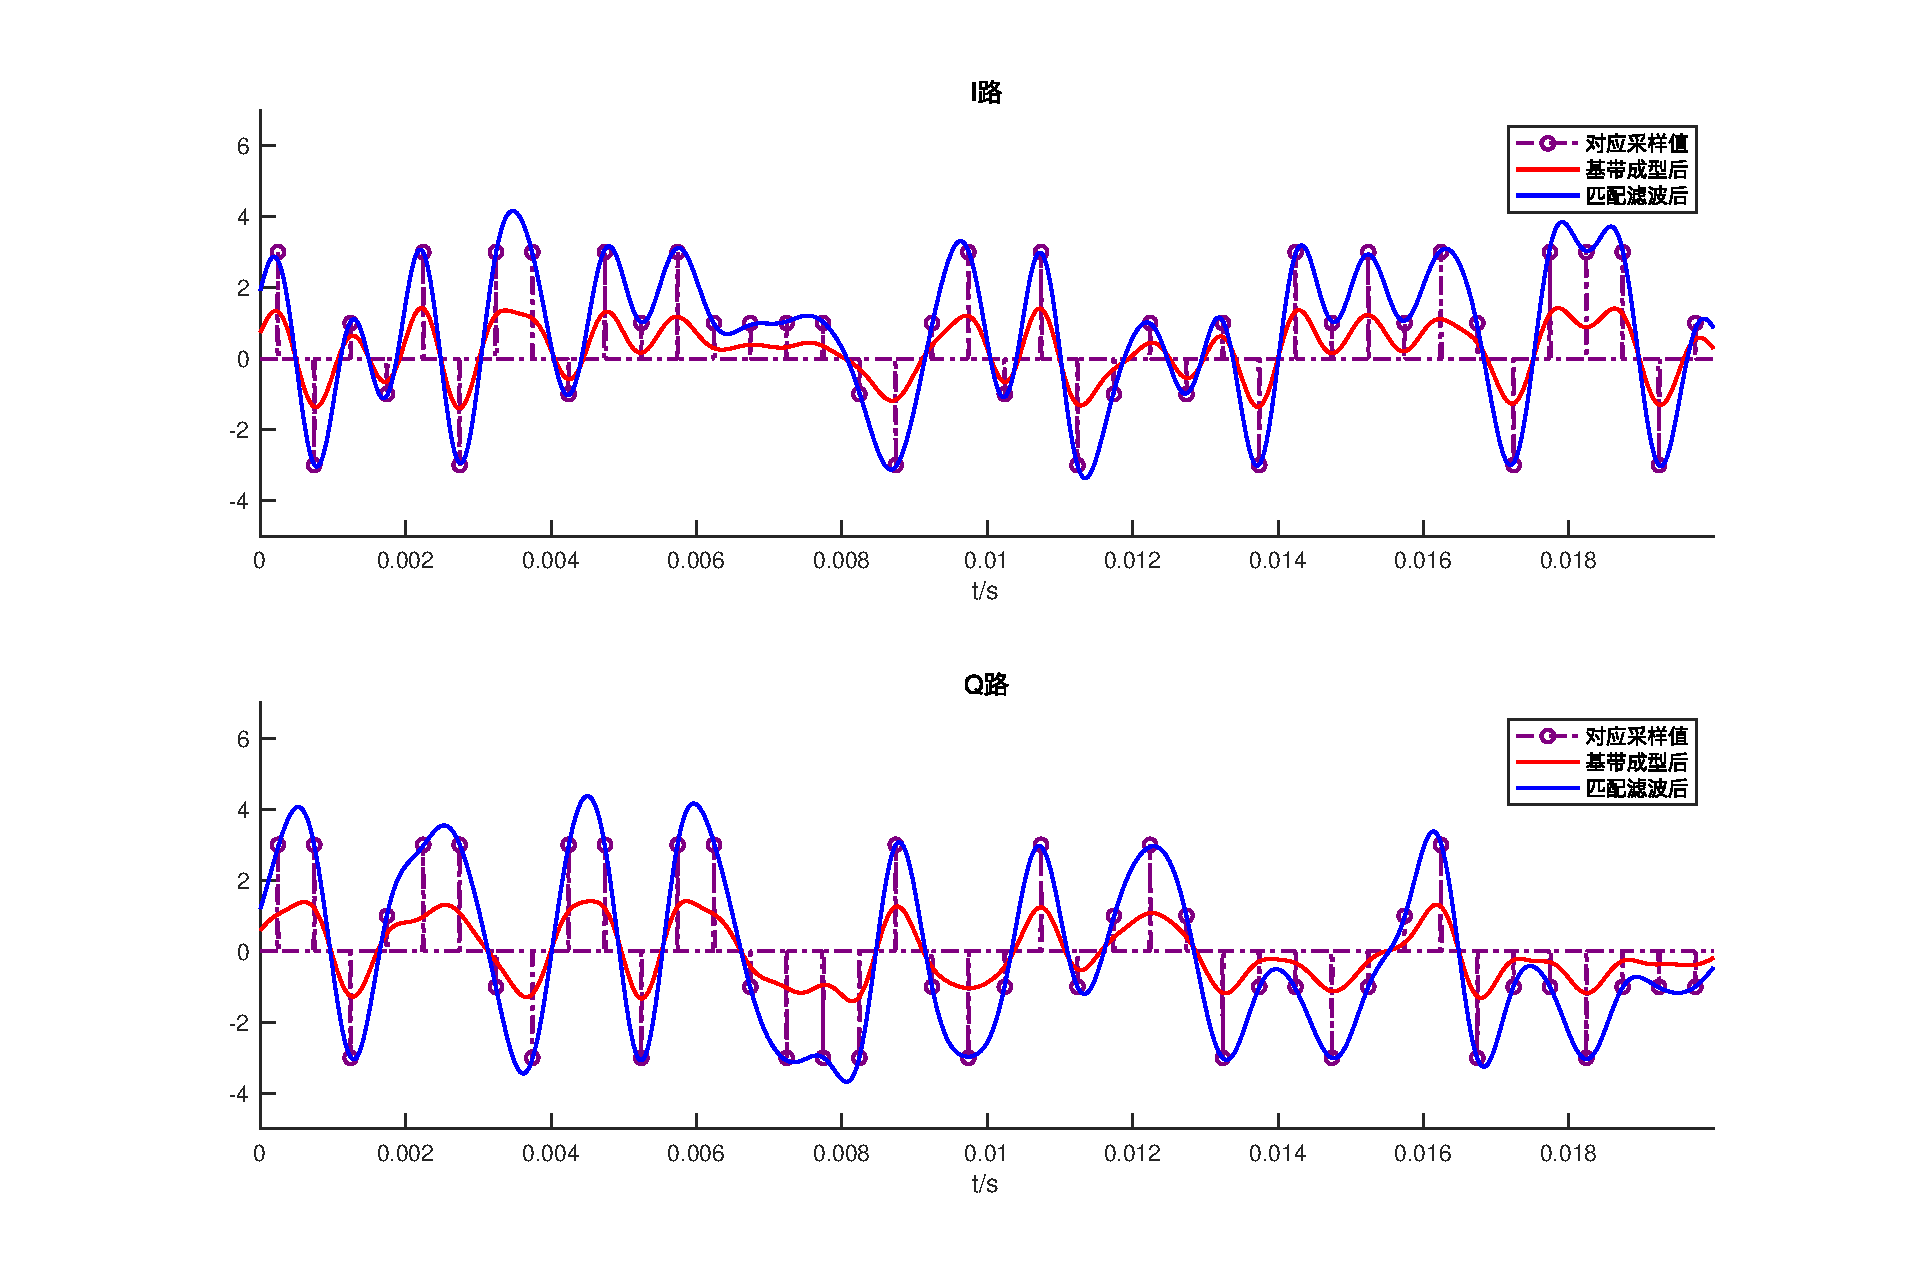
\includegraphics[width=0.8\textwidth]{./pic/sample.eps}
    \caption{最佳采样点的采样结果}
\end{figure}

\subsection{信道实现}

对于波形信道而言,各种传输方案的信噪比最终都是以$\frac{E_b}{n_0}$的形式来加以比较的,其中$E_b$代表每比特对应的能量,而$n_0$则对应双边功率谱密度,因为复数电平需要I路和Q路两路调制。在各种映射方式中,为了降低误码率,都采用了格雷码映射的方式,一个电平符号发生的错误可以近似地认为只会引发一比特的错误,进而在M元映射时有
\begin{equation*}
P_b=\frac{P_s}{\log_2M}
\end{equation*}

在明确了误比特率和误符号率的关系之后,可以直接考虑电平符号能量与噪声功率谱密度之间的关系,即$\frac{E_s}{n_0}$。理想的波形信道中的信号应该是连续的,但实际上仿真出的波形信道是离散的,由于采样率有限,可以等效为一个低通系统,带宽即为采样率的二分之一。在这种情况下,实际添加的噪声不可能是理想的高斯白噪声,在整个频谱上的取值均为常数,而只可能是在有限的频带内为常数。因此噪声对应的总能量应为
\begin{equation*}
N=\frac{f_s}{2}\cdot\frac{n_0}{2}=\frac{f_sn_0}{4}
\end{equation*}

对于信号的能量$E_s$,在信号满足宽平稳的假设下,可以得到
\begin{equation*}
E_s=\frac{\int_{0}^{T_s}E|X^2(t)|dt}{T_s}=f_s\int_{0}^{T_s}E|X^2(t)|dt
\end{equation*}

其中X(t)对应的是基带信号的幅值。由于每个符号对应的基带成型波形都是同样的升余弦滚降滤波函数,因此可以根据帕塞瓦尔方程得到
\begin{equation*}
E_s=\frac{\int_{0}^{T_{symbol}}E|X^2(t)|dt}{T_{symbol}}=\frac{E(|a|^2)\int_{-\infty}^{+\infty}|G(f)|^2df}{T_{symbol}}=\frac{E(|a|^2)\int_{0}^{T_{symbol}}|g(t)|^2dt}{T_{symbol}}
\end{equation*}

上式中的$\int_{0}^{T_{symbol}}|g(t)|^2dt$表示基带成型滤波器在一个码元周期内对应的归一化能量。但是在实际的仿真中,信号的波形也是用离散值逼近出来的。因此有
\begin{equation*}
E_s=E(|a|^2)T_s\sum\limits_{n=0}^{N-1}|g(t-nT_s)|^2, N=\frac{T_{symbol}}{T_s}
\end{equation*}

MATLAB的rcosdesign()函数给出的波形对应结果为$\sum\limits_{n=0}^{N-1}|g(t-nT_s)|^2=1$,因此电平符号能量可以进一步简化
\begin{equation*}
E_s=E(|a|^2)T_s=\frac{E(|a|^2)}{f_s}
\end{equation*}

从而推导得到仿真中噪声序列的方差
\begin{equation*}
N=\frac{f_sn_0}{4}=\frac{f_sE_s}{4(\frac{E_s}{n_0})}=\frac{E(|a|^2)}{4(\frac{E_s}{n_0})}
\end{equation*}

为了验证上述推到的正确性,可以选择几种典型的映射方式进行考察,下图是2ASK, BPSK, QPSK和16QAM理论计算和仿真得到误符号率曲线比较,可以看到除了16QAM在低信噪比下误符号率公式不成立,以及高信噪比下误符号率较低引起的波动以外,其他部分得到的仿真值基本都与理论值完全一致。

\begin{figure}[h]
    \centering
    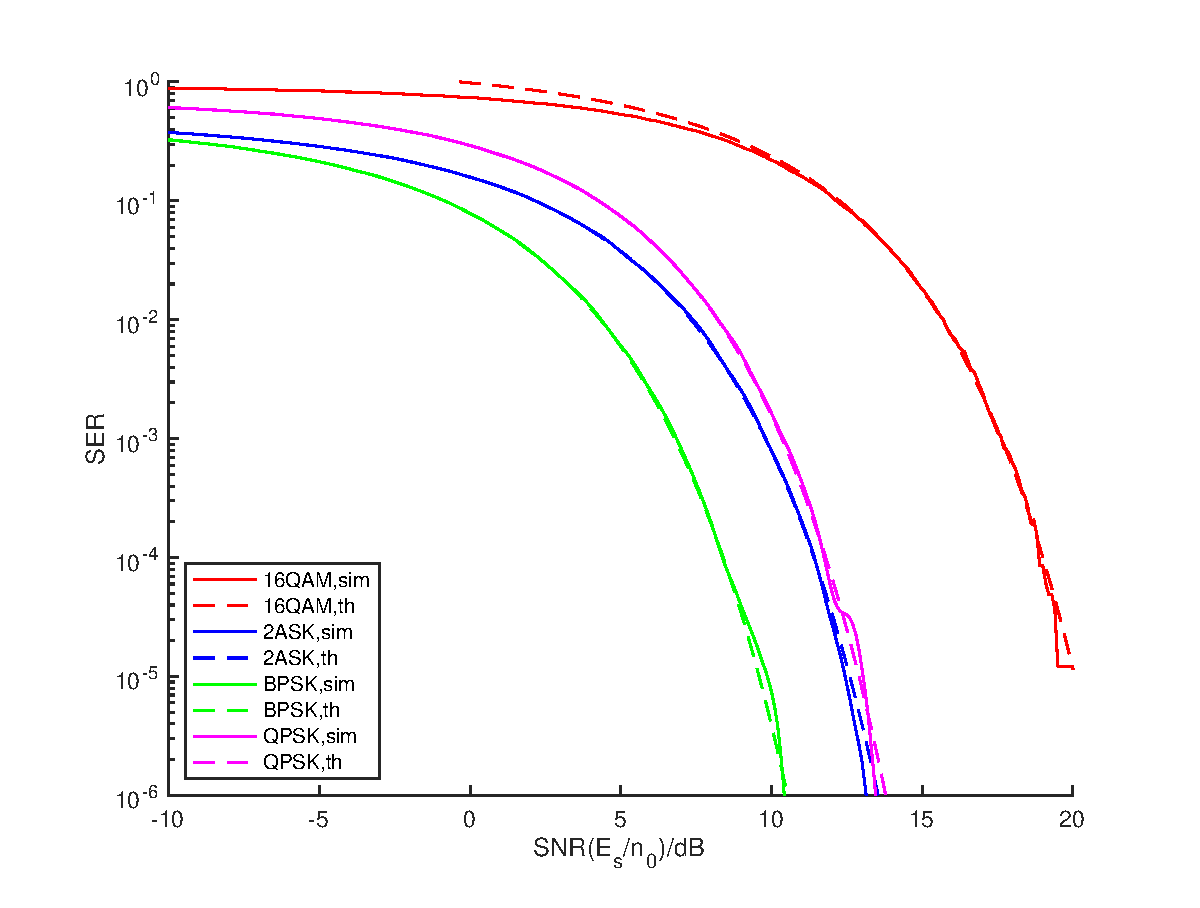
\includegraphics[width=0.4\textwidth]{./pic/SNR_SER.eps}
    \caption{几种映射方式理论值和仿真值的SNR-SER曲线}
\end{figure}

\subsection{信道编码}

\subsubsection{卷积码}

本次实验中的卷积码模块基本与上次实验中的一致,只不过根据不同的映射方式对软判决模块的欧氏距离累计进行了调整。下图是卷积码在波形信道中的仿真结果,仿真中依旧选取了四种典型的映射方式,分别考察了在不进行卷积码编码、硬判决、软判决三种情况下的性能。可以看到软判决的性能还是明显优于硬判决的,而在低信噪比的情况下卷积码的性能比不进行编码差,但在高信噪比的情况下恰好相反。这样的结果与电平信道的仿真结果一致,说明之前适用于电平信道的卷积码的编解码模块同样适用于波形信道。

\begin{figure}[h]
    \centering
    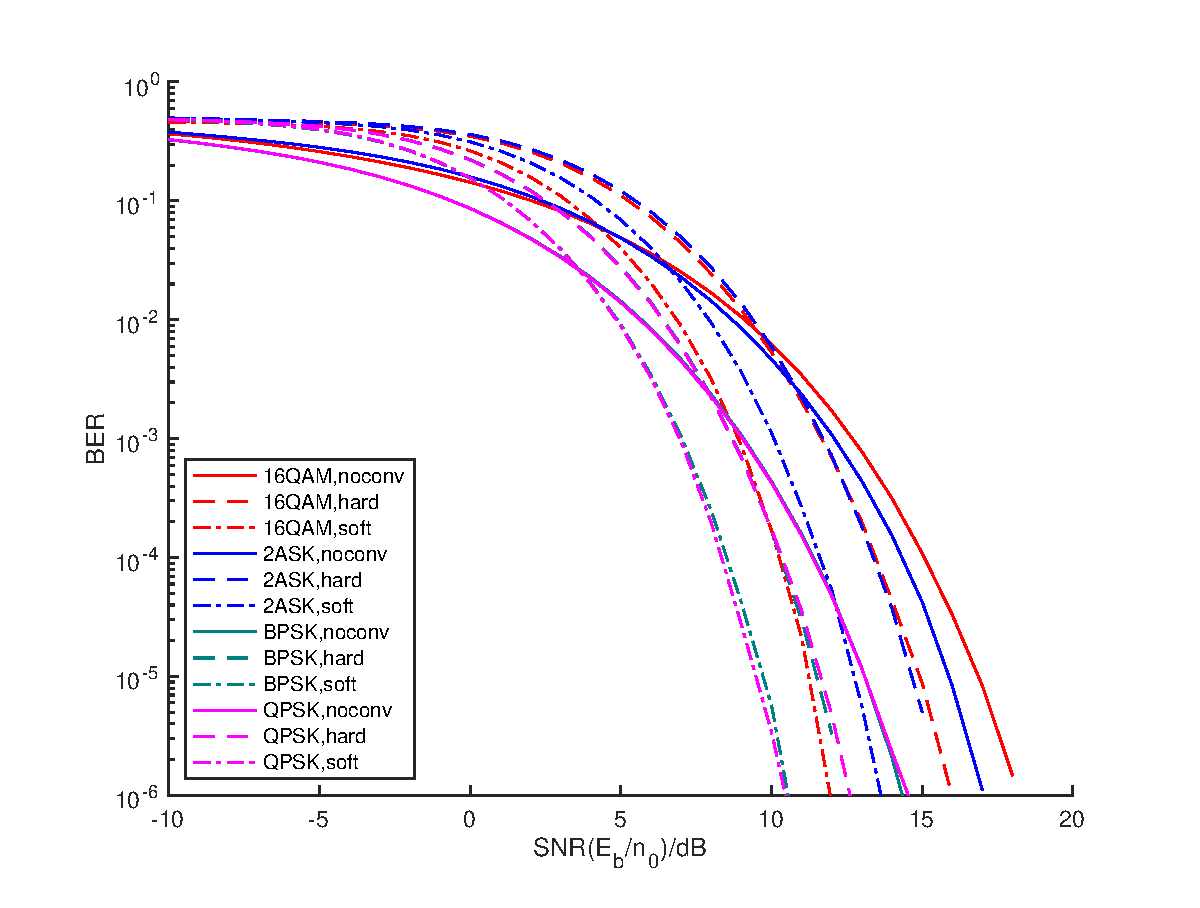
\includegraphics[width=0.4\textwidth]{./pic/conv_SNR_BER.eps}
    \caption{几种映射方式在不进行卷积码编码、硬判决、软判决下的SNR-BER曲线}
\end{figure}


\subsubsection{里德-索罗蒙码}

除了卷积码以外,本次实验还尝试了分组码的方法,这里实现的是里德-索罗蒙码,即R-S码。这是一种可非二进制循环码,码元由m个比特组成,其中m$>$2,m比特码元对应R-S(n,k)码,其中n为分组中的总码元数,k为分组中的信息码元数,2t=n-k为分组中的监督码元数,t为能纠正的错误码元个数。R-S码最显著的特征是可以有效对抗突发噪声,因为非二进制的特性,即使比特流中有很长的一连串受到影响,对应码元的个数也可能很小,进而被纠正过来。

R-S码的编码比较简单,对于待编码的二进制流,先通过串并转换将转换为对应的多进制流,再进行分组,对于每组的k个信息码元,可以先表示成有限域上多项式的形式。之后先统一乘以 $X_{2t}$,再除以规定好的本原多项式,2t位的商多项式既可作为监督码元。
    
与卷积码相比,R-S码的解码则较为复杂一些,但基本思路与一般分组码的译码类似。对于一个码组,先计算出校正子,再确定出错误位置多项式,但与二进制分组码不同的是,在寻找到错误位置以后,由于是多进制码,错误值有多种选择,因此不能像二进制分组码一样在错误位置进行简单的反转,而应该根据校正子方程计算出错误取值,才能对码组进行纠正。由于整个译码的过程略显冗繁,在此不做更详细的介绍。

下图为采用BPSK映射方式时不进行R-S编码和进行R-S(7,3)编码的信噪比-误比特率曲线。 可以看到在相同的$\frac{E_b}{n_0}$的情况下,不进行R-S编码的性能反而要比进行R-S编码的性能好,这样的结果是令人失望的。但是从曲线的走势可以看出,R-S编码对应的曲线在高信噪比的条件时似乎有更陡峭的下降趋势,因此有可能以更快的速度达到更小的差错概率,但是受计算机性能的限制,很难再提高仿真的规模。

\begin{figure}[h]
    \centering
    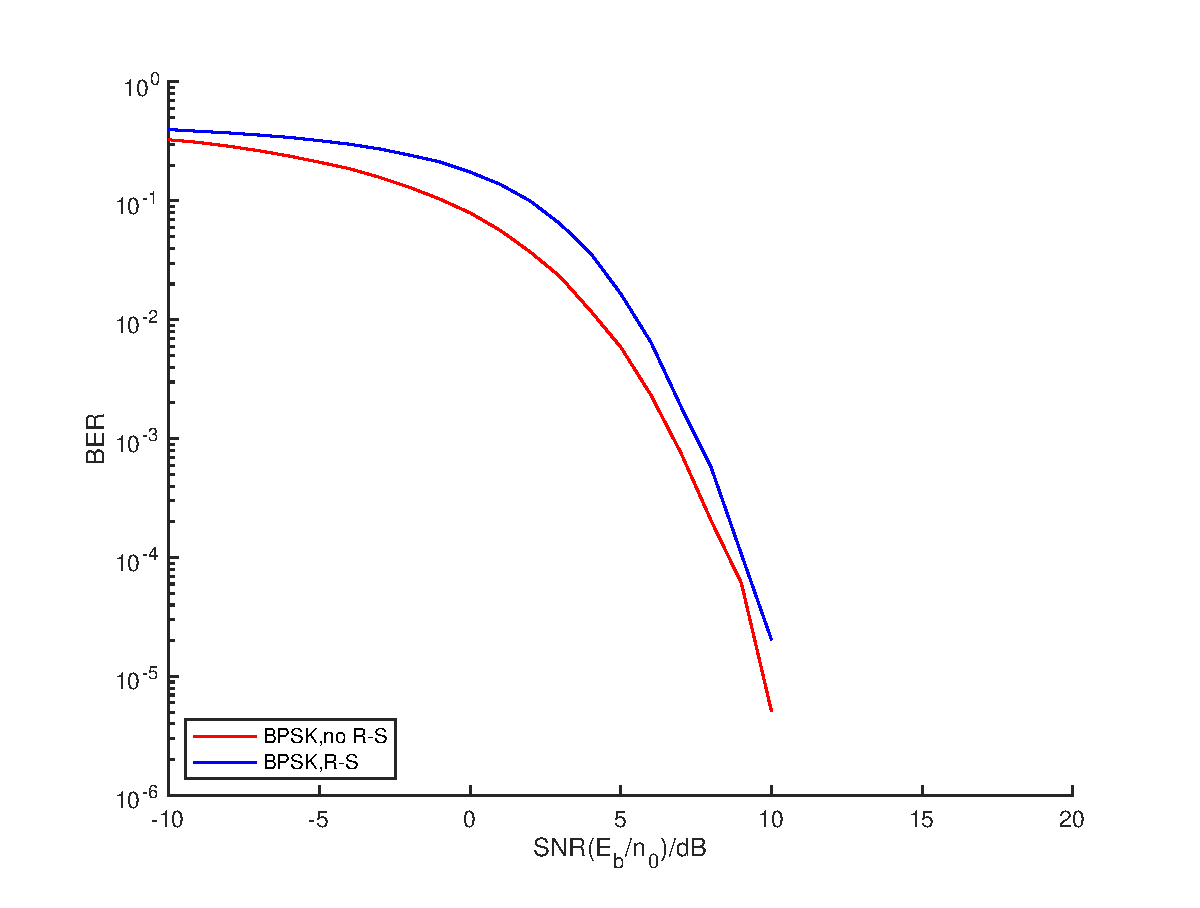
\includegraphics[width=0.45\textwidth]{./pic/RS_SNR_BER.eps}
    \caption{不进行与进行R-S编码的SNR-BER曲线}
\end{figure}

\subsection{整体方案设计}

由于仿真中并没有能得出R-S编码的有效性,最后的传输方案本质上仍然只是不同效率卷积码和不同映射方式的匹配。通过比较多种匹配方案,最终选择了QPSK搭配$\frac{1}{2}$效率卷积码的方案,其功率谱如下。
\begin{figure}[h]
    \centering
        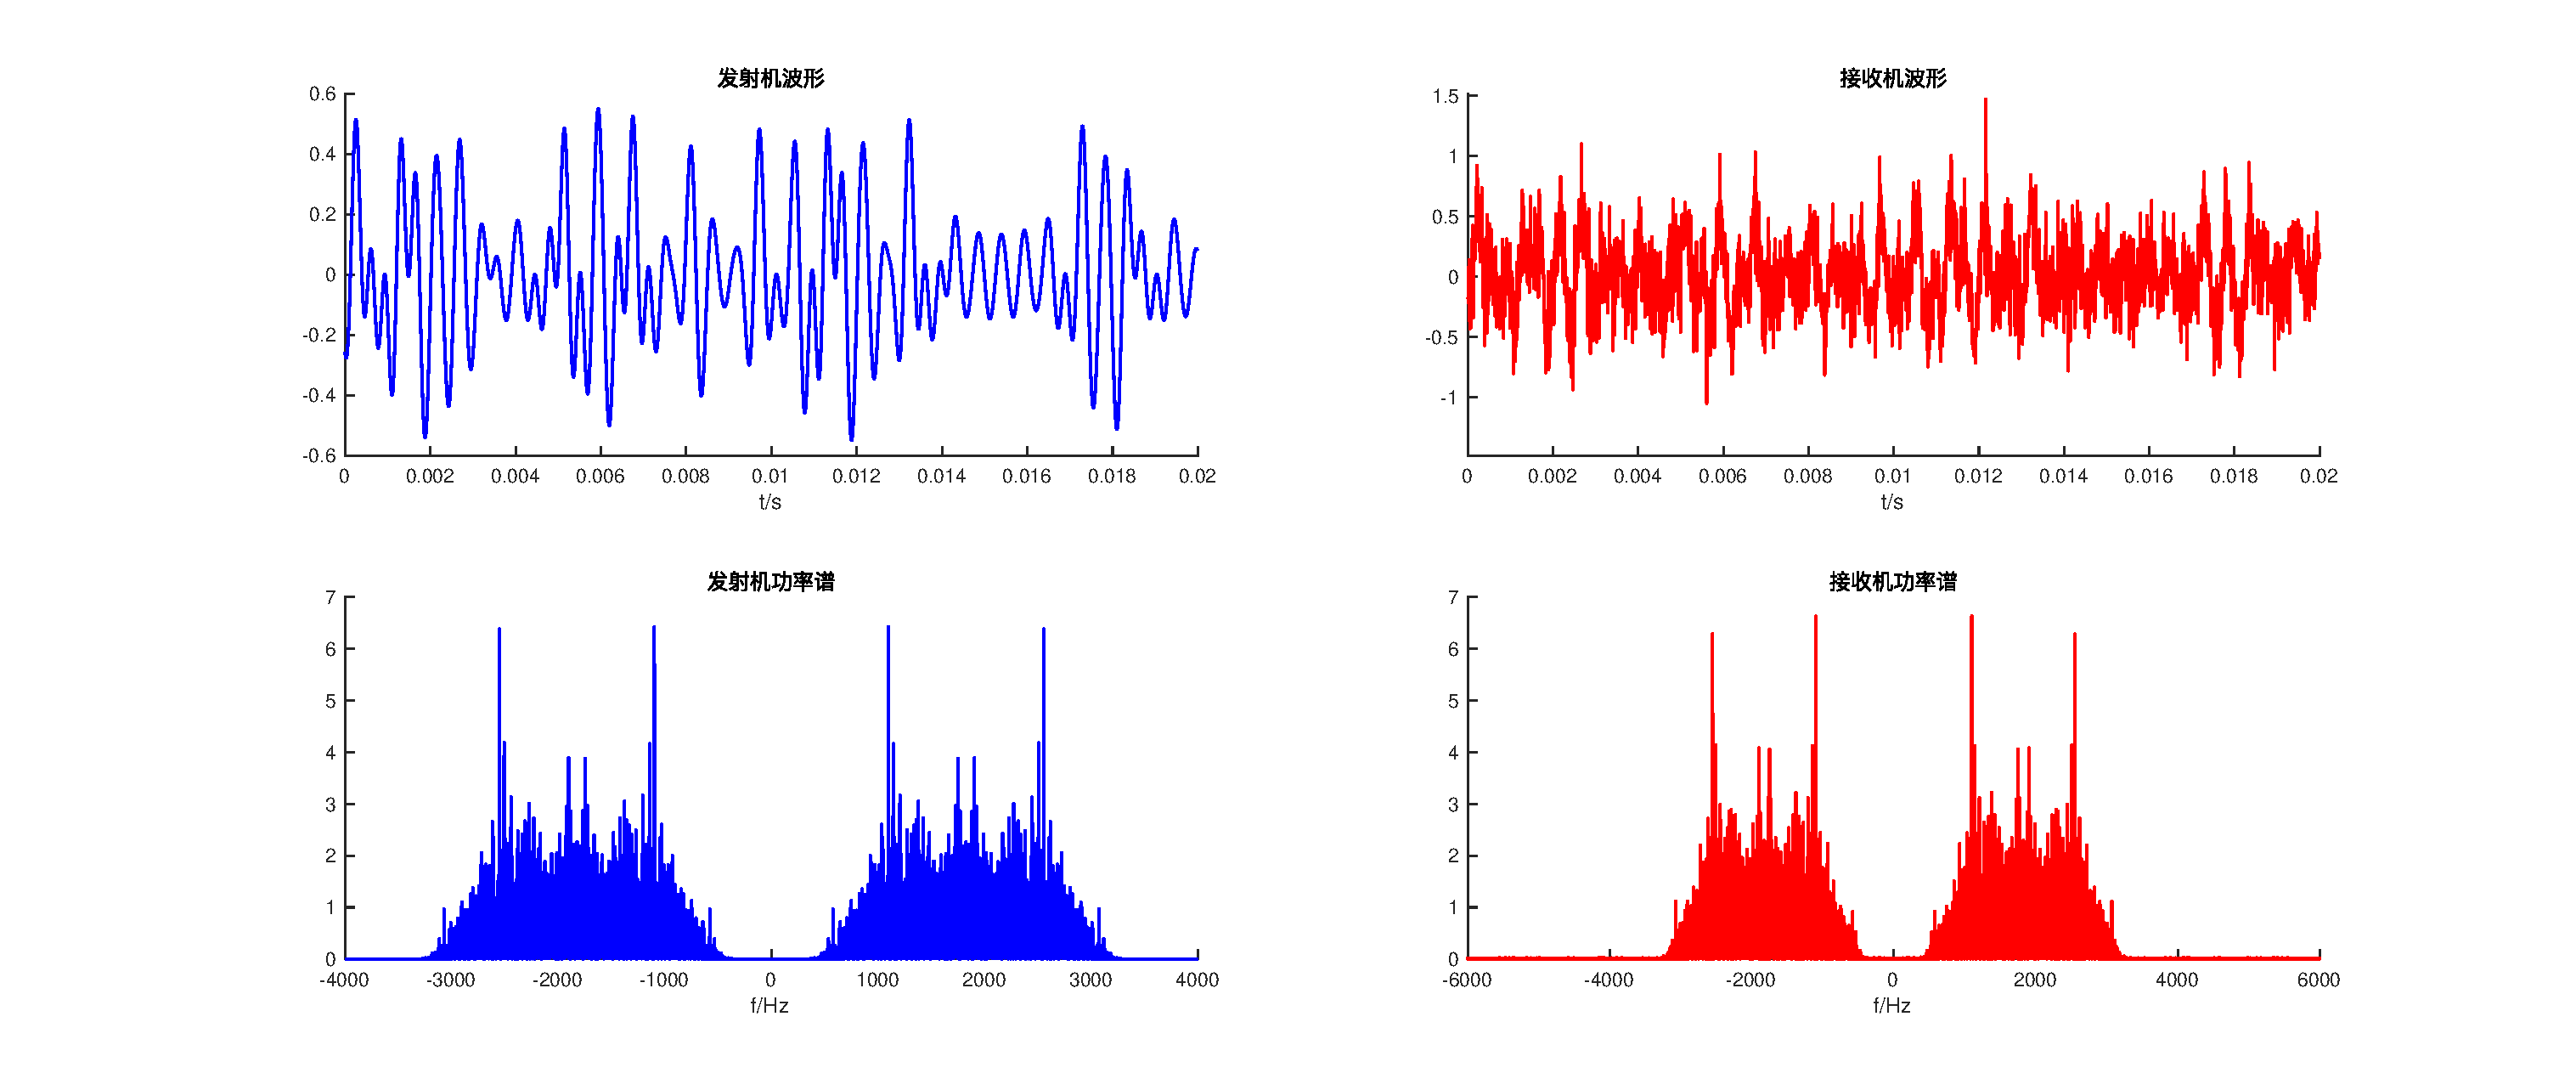
\includegraphics[width=\textwidth]{./pic/transmit.eps}
    \caption{整体传输方案的波形及功率谱}
\end{figure}

以这种传输方案传输1kByte的数据,共发送8000个电平符号,在$R_s$=2000Baud的符号率的条件下,总传输时间约为4s,满足要求。

\section{AES密码}

AES(Advanced Encryption Standard)是一种常用的对称加密算法,其基本思想是设计一个代换与置换组合的网络(substitution-permutation network),在硬件和软件层面都有较好的性能。AES加解密的整体流程如下图所示。

\begin{figure}[h]
    \centering
    \includegraphics[width=\textwidth,trim=0 20 0 20,clip]{./pic/AES_flow.eps}
    \caption{AES加解密整体流程}
\end{figure}

AES密码为分组密码,它先将明文分为128 bits的若干组,然后对每一组进行代换置换结合的多轮加密,直到加密完整个明文。AES的密钥长度为128,192,或256 bits,对于不同的密钥长度L=length(key),我们定义Nk为密钥中32-bit字的个数,即Nk=L/32;由Nk我们可以获得加密轮数Nr=Nk+6。不同密钥长度对应的Nk与Nr值如下表所示

\begin{table}[h]
    \centering
    \begin{tabular}{|c|c|c|c|}
        \hline
        \textbf{L} & 128 bits & 192 bits & 256 bits \\
        \hline
        \textbf{Nk} & 4 & 6 & 8 \\
        \hline
        \textbf{Nr} & 10 & 12 & 14 \\
        \hline
    \end{tabular}
    \caption{不同密钥长度对应的Nk, Nr值}
\end{table}

下面主要讨论AES加解密中密钥扩展,加密模块,解密模块和仿真分析。

\subsection{密钥扩展}

AES的加解密过程中需要进行多轮的代换置换操作,而在每一轮操作中都需要一个长度为 128 bits的轮密钥roundKey,因此我们首先需要将长度为32Nk bits的初始密钥key扩展为长度为 128(Nr+1) bits的多轮密钥W。

\subsubsection{初始处理}

将初始密钥key重构为一个4$\times$Nk的矩阵,这里的每个矩阵元素长度均为1 byte(8 bits),这个矩阵即为多轮密钥W的前Nk列元素。以长度为128 bits的密钥为例,其初始处理操作如下图所示

\begin{figure}[h]
    \centering
    \includegraphics[width=0.65\textwidth]{./pic/keyExpansion_1.eps}
    \caption{128 bits密钥的初始处理}
\end{figure}

\subsubsection{递推迭代}

在得到了W的前Nk列元素后,我们就可以用迭代的方式获得其余的各列元素。设当前列号为cnt,则该列元素的迭代方式为
\begin{enumerate}
    \item 若cnt$\equiv$1 (mod Nk),则W[cnt]=W[cnt-Nk]$\oplus F_1$(W[cnt-1]);
    \item 若Nk=8且cnt$\equiv$5 (mod Nk),则W[cnt]=W[cnt-Nk]$\oplus F_2$(W[cnt-1]);
    \item 否则,W[cnt]=W[cnt-Nk]$\oplus$W[cnt-1]。
\end{enumerate}

其中$F_1$(K)=subWord(rotWord(K))$\oplus$Rcon[(cnt-1)/k]; $F_2$(K)=subWord(K); $\oplus$表示按位异或。下面简要说明subWord()函数,rotWord()函数,和Rcon[ ]常量。

subWord()函数计算输入值K的每一个分量在$GF(2^8)$域上逆的一个仿射变换,其本质是一个非线性的置换操作,在实际中通过查表高效地实现。详细讨论见\ref{subBytes}。

rotWord()函数将输入值K的4个字节循环左移1个字节。如若输入$K_{in}=[k_1,k_2,k_3,k_4]'$,则输出为$K_{out}=[k_2,k_3,k_4,k_1]'$。

Rcon[ ]为一个4字节的常量,可表示为$Rcon_i$=[$Rc_i$,0x00,0x00,0x00],其中Rc[ ]的取值为

\begin{table}[h]
    \centering
    \begin{tabular}{|c|c|c|c|c|c|c|c|c|c|c|}
        \hline
        \textbf{i} & 1 & 2 & 3 & 4 & 5 & 6 & 7 & 8 & 9 & 10 \\
        \hline
        \textbf{Rc$_i$} & 0x01 & 0x02 & 0x04 & 0x08 & 0x10 & 0x20 & 0x40 & 0x80 & 0x1b & 0x36 \\
        \hline
    \end{tabular}
    \caption{Rc的取值}
\end{table}

以长度为128 bits的密钥为例,其最初4次迭代过程如下图所示

\begin{figure}[h]
    \centering
    \includegraphics[width=0.5\textwidth]{./pic/keyExpansion_2.eps}
    \caption{128 bits密钥的递推迭代}
\end{figure}

\subsection{加密模块}

加密模块的核心是encrypt()函数,它以128 bits的明文plaintext和经过扩展后的多轮密钥W 为输入,经过多轮可逆的代换置换操作输出128 bits的密文cyphertext。具体加密流程如下图所示

\begin{figure}[h]
    \centering
    \includegraphics[width=0.9\textwidth,trim=0 30 0 20,clip]{./pic/encrypt.eps}
    \caption{encrypt()函数加密流程}
\end{figure}

\begin{enumerate}
    \item 将明文重构为一个4$\times$4的矩阵中,其每个元素长度均为1 byte(8 bits),我们将这个矩阵称为状态矩阵;
    \item 对状态矩阵进行轮密钥加addRoundKey();
    \item 对状态矩阵进行Nr-1轮代换置换操作,具体步骤为
    \begin{enumerate}
        \item 字节代换subBytes();
        \item 行移位shiftRows();
        \item 列混合mixColumns();
        \item 轮密钥加addRoundKey();
    \end{enumerate}
    \item 对状态矩阵进行最后1轮字节代换,行移位,和轮密钥加;
    \item 将经Nr轮代换替换操作后的状态矩阵重构为128 bits的密文。
\end{enumerate}

下面分别说明每轮代换置换中用到的各个函数。

\subsubsection{subBytes()}
\label{subBytes}

subBytes()函数将状态矩阵的每个元素替换为其在$GF(2^8)$域上逆的一个仿射变换。在实际中通过一个查找表S-Box(具体取值见表\ref{S-Box})来高效地实现。subBytes()本质上是一个置换操作,它为AES密码提供了良好的非线性,从而避免了基于代数性质的攻击。subByte() 函数的执行过程如下图所示

\begin{figure}[h]
    \centering
    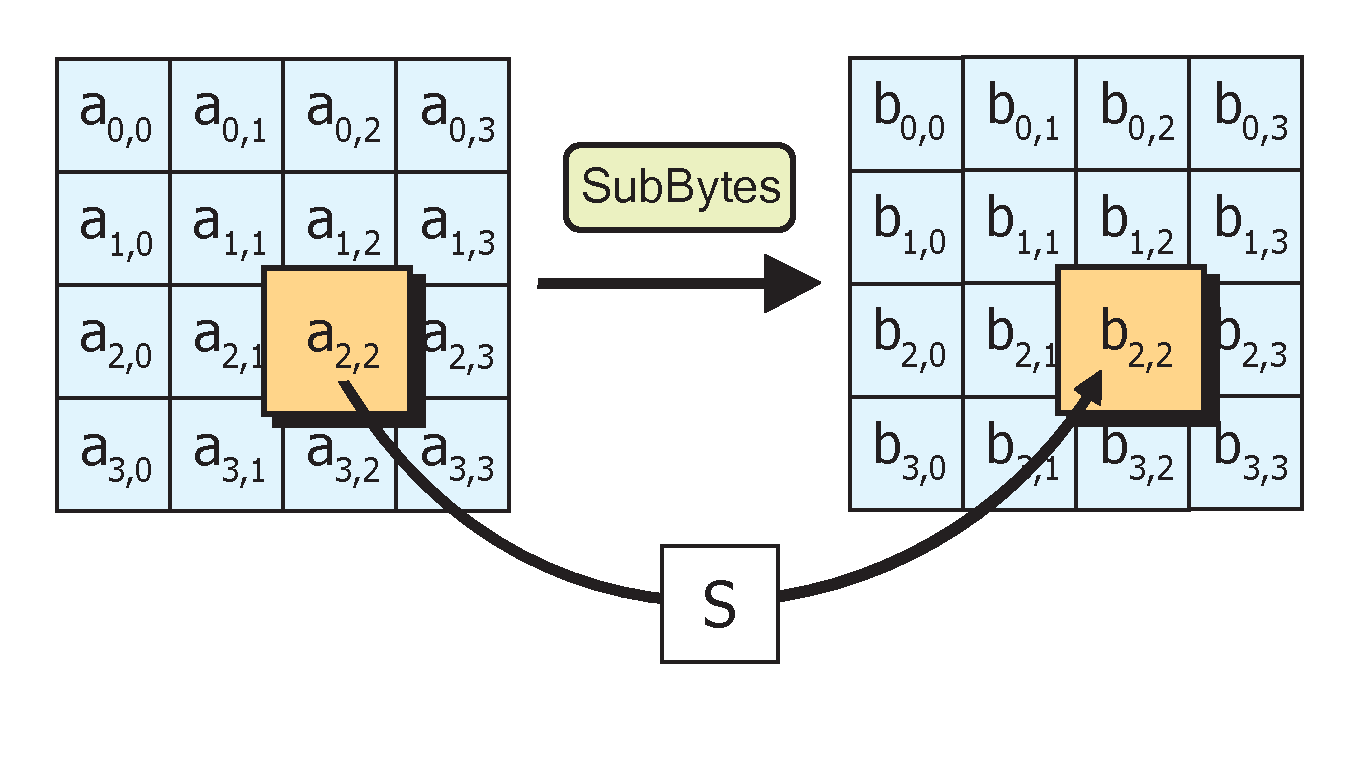
\includegraphics[width=0.4\textwidth,trim=0 30 0 10,clip]{./pic/subBytes.eps}
    \caption{subBytes()函数}
\end{figure}

\subsubsection{shiftRows()}

shiftRows()函数对状态矩阵每一行的4个字节进行固定字节数的循环左移。具体而言,状态矩阵的第1行保持不变;第2行循环左移1个字节;第3行循环左移2个字节;第4行循环左移3个字节。shiftRows()函数的执行过程如下图所示

\begin{figure}[h]
    \centering
    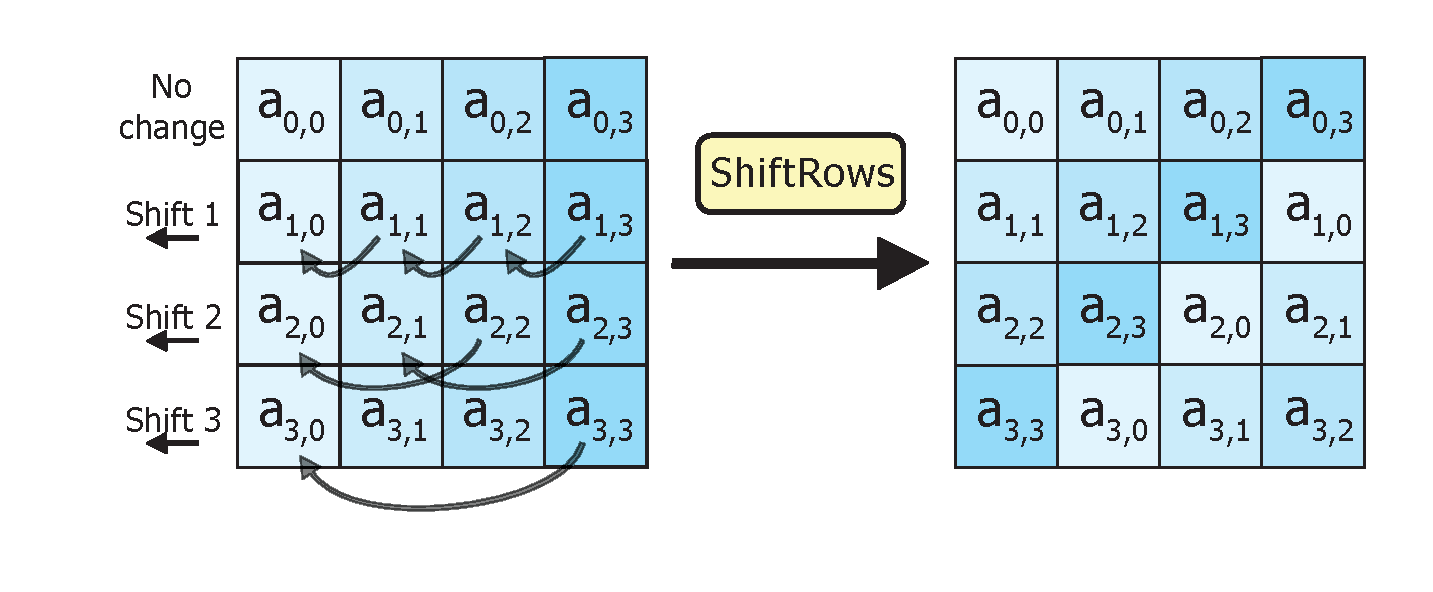
\includegraphics[width=0.5\textwidth,trim=0 30 0 10,clip]{./pic/shiftRows.eps}
    \caption{shiftRows()函数}
\end{figure}

\subsubsection{mixColumns()}

mixColumns()函数对状态矩阵进行一个可逆的线性变换,从而实现状态矩阵的列混合。具体而言,是对状态矩阵左乘一个固定的矩阵C(具体取值见式(\ref{C})),注意到这里的乘法和加法都是定义在$GF(2^8)$域上的运算,在实际中为了提高效率通过查找表实现。mixColumns()函数的执行过程如下图所示

\begin{figure}[h]
    \centering
    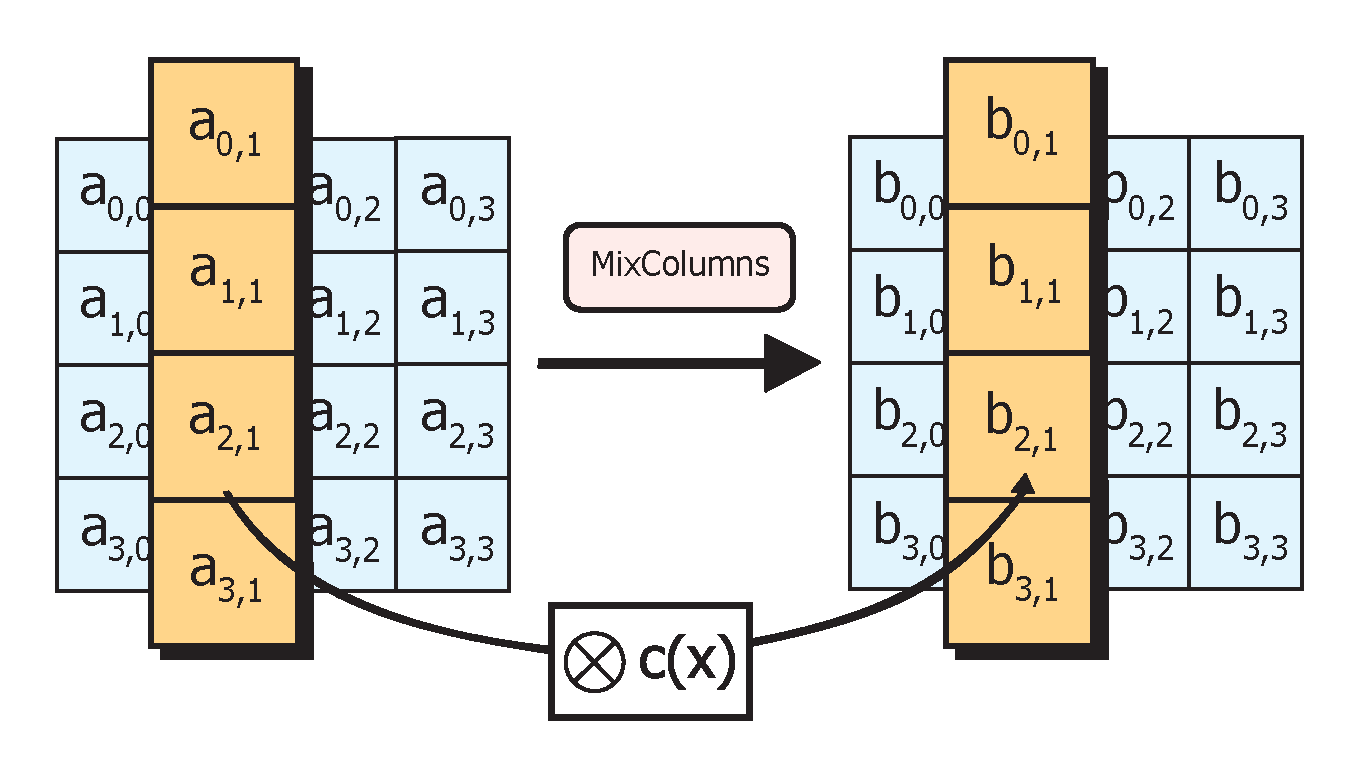
\includegraphics[width=0.4\textwidth,trim=0 20 0 0,clip]{./pic/mixColumns.eps}
    \caption{mixColumns()函数}
\end{figure}

\subsubsection{addRoundKey()}

addRoundKey()函数将状态矩阵与轮密钥进行按位异或,从而实现明文信息与密钥信息的混合。注意到按位异或是可逆的,其逆操作也是按位异或,故在解密函数中同样需要使用该函数,之后不再赘述。addRoundKey()函数的执行过程如下图所示

\begin{figure}[h]
    \centering
    \includegraphics[width=0.4\textwidth,trim=0 10 0 0,clip]{./pic/addRoundKey.eps}
    \caption{addRoundKey()函数}
\end{figure}

\subsection{解密模块}

加密模块的核心是decrypt()函数,它以128 bits的密文cyphertext和经过扩展后的多轮密钥W 为输入,对应于encrypt()函数的多轮加密过程,进行多轮代换置换的逆操作,输出128 bits的明文plaintext。具体解密流程如下图所示

\begin{figure}[h]
    \centering
    \includegraphics[width=0.9\textwidth,trim=0 30 0 20,clip]{./pic/decrypt.eps}
    \caption{decrypt()函数解密流程}
\end{figure}

\begin{enumerate}
    \item 将密文重构为4$\times$4的状态矩阵;
    \item 对状态矩阵进行轮密钥加addRoundKey();
    \item 对状态矩阵进行Nr-1轮代换置换操作,具体步骤为
    \begin{enumerate}
        \item 逆行移位iShiftRows();
        \item 逆字节代换iSubBytes();
        \item 轮密钥加addRoundKey();
        \item 逆列混合iMixColumns();
    \end{enumerate}
    \item 对状态矩阵进行最后1轮逆行移位,逆字节代换,和轮密钥加;
    \item 将经Nr轮代换替换操作后的状态矩阵重构为128 bits的明文。
\end{enumerate}

每轮解密过程中用到的各函数即为加密过程中用到的可逆函数对应的逆函数,下面简要说明。

\subsubsection{iSubBytes()}

iSubBytes()函数将状态矩阵的各元素替换为其在S-Box中的原象。在实际中通过iS-Box查找表(具体取值见表\ref{iS-Box})高效地实现。

\subsubsection{iShiftRows()}

iShiftRows()函数对状态矩阵每一行的4个字节进行固定字节数的循环右移。具体而言,状态矩阵的第1行保持不变;第2行循环右移1个字节;第3行循环右移2个字节;第4行循环右移3个字节。

\subsubsection{iMixColumns()}

iMixColumns()函数对状态矩阵左乘固定矩阵C在$GF(2^8)$域上的逆矩阵(具体取值见式(\ref{iC})),在实际中通过查找表高效地实现。

\subsection{仿真分析}

在仿真分析中,我们对比了三种不同的通信方式:

\begin{enumerate}
    \item 第一种通信方式(no AES)不进行加解密,采用1/2效率的卷积编码,4PSK的电平映射,和滚将系数$\alpha$=0.5的升余弦滚降滤波器,信道为AWGN信道;
    \item 第二种通信方式(AES conv)在第一种通信方式的基础上进行了AES加解密,在发端采用先加密后卷积的组合顺序,其余模块完全相同;
    \item 第三种通信方式(conv AES)也是在第一种通信方式的基础上进行了AES加解密,与第二种通信方式的区别是在发端采用先卷积后加密的组合顺序,其余模块完全相同
\end{enumerate}

三种通信方式仿真得到的BER-SNR曲线如图所示,其中左边的图为线性坐标,右边的图为对数坐标。

\begin{figure}[h]
    \centering
    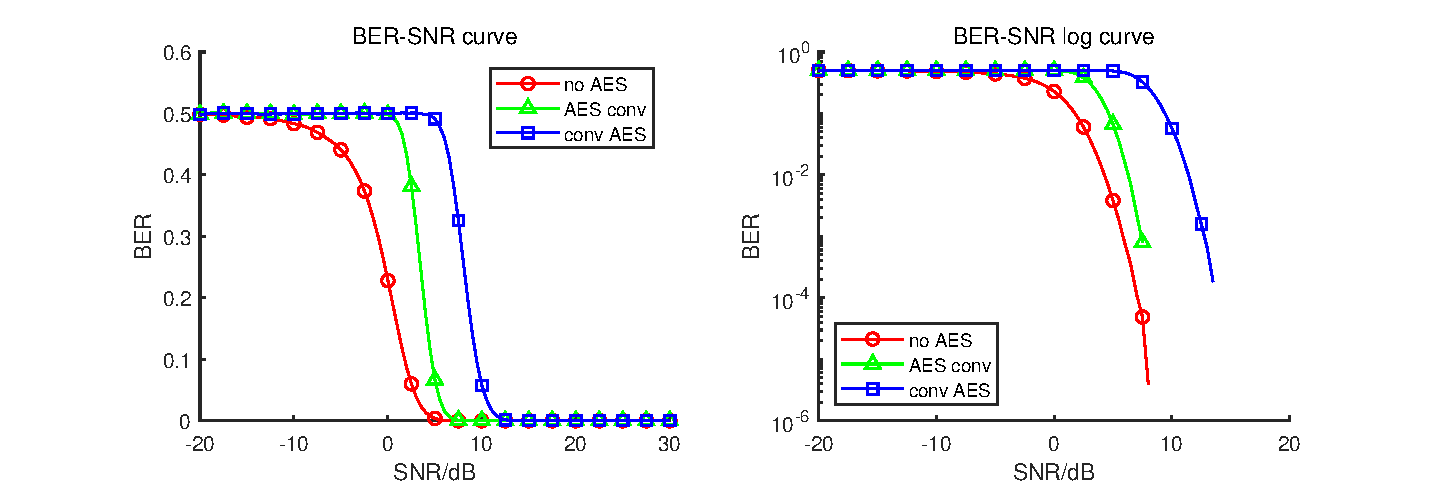
\includegraphics[width=\textwidth]{./pic/AES_sim.eps}
    \caption{conv, AES conv和conv AES的BER-SNR曲线}
\end{figure}

\paragraph{}结合仿真结果和理论分析,我们可以得到如下两条结论。

\paragraph{结论1}密码模块以通信的可靠性为代价提高了通信的安全性。

对比图中不进行加密的红线和进行加密的绿线及蓝线可以看出,在相同信噪比的条件下,不进行加密的误码率低于进行加密的误码率。

从原理上进行分析,这是因为密码模块通常具有扩散效应,即明文中的一个符号变化就能导致密文中大量符号的变化,从而导致在密文只有少量错误码字时,解密出的明文却存在大量错误的码字;而从安全性的角度考虑,扩散效应能够防止密码在受到选择性明文攻击时被轻易地破译。因此,密码设计中的扩散原则实际上是以通信的可靠性为代价提高了通信的安全性。

注意到对数坐标的图中,先加密后卷积的绿线与不加密的红线性能较为接近,在信噪比为 10dB时能得到不超过$10^{-4}$的误码率。考虑到进行AES密码较强的防攻击性能,我们认为以部分通信可靠性为代价显著提升通信安全性的方案是可以接受的。

\paragraph{结论2}加密模块应在信道编码模块之前。

从可靠性的角度考虑,对比图中先加密后卷积的绿线和先卷积后加密的蓝线可以看出,在相同信噪比的条件下,先加密的误码率低于先卷积的误码率。这是因为卷积码具有记忆特性:在先加密后卷积的通信方式中,收端可以先通过卷积码译码纠出一部分的错误,从而减少解密过程中由于扩散而导致的错误码字;而在先卷积后加密的通信方式中,由于密码的扩散效应,收端在通过解密模块后误码率会大大增加,尽管卷积码译码可以纠出部分错误,但与增加的错误码字相比仍是少数,且在误码率本身较高的情况下,卷积码的记忆特性甚至会导致原本正确的码字被连带地判为错误的码字,从而导致误码率大大增加。

从安全性的角度考虑,在面对惟密文攻击时,我们希望明文中包含的冗余信息越少越好。这是因为在Eve可能获得大量明文密文对的情况下,明文中的冗余信息越少,Eve破译出密钥的难度就越大。而卷积码编码等信道编码本质上就是通过引入冗余提高通信的可靠性,因此在引入冗余前就进行加密能够有效提高通信的安全性。

\paragraph{}
在不同信噪比下,有加密与无加密的25-bit误码图案对比如下,其中白色代表正确码字,黑色代表错误码字。图中的误码图案也反映出了AES密码的扩散效应。

\begin{figure}[h]
    \centering
    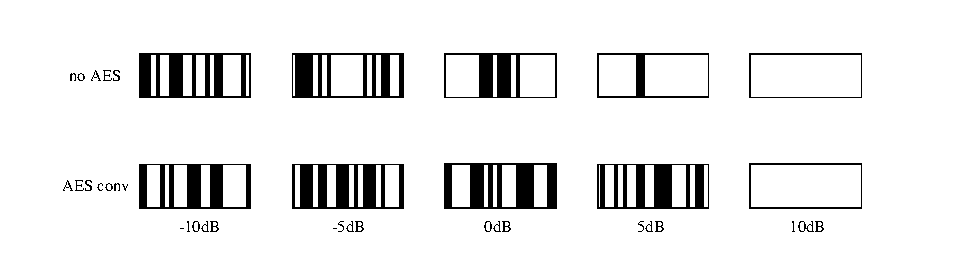
\includegraphics[width=\textwidth,trim=0 5 0 15,clip]{./pic/AES_pattern.eps}
    \caption{不同信噪比条件下有无加密时的25-bit误码图案}
\end{figure}

\subsection*{AES密码附录}

\subsubsection*{S-Box}

\begin{table}[h]
    \centering
    \begin{tabular}	{|c|c|c|c|c|c|c|c|c|c|c|c|c|c|c|c|c|}
        \hline
        & \textbf{00} & \textbf{01} & \textbf{02} & \textbf{03} & \textbf{04} & \textbf{05} & \textbf{06} & \textbf{07} & \textbf{08} & \textbf{09} & \textbf{0a} & \textbf{0b} & \textbf{0c} & \textbf{0d} & \textbf{0e} & \textbf{0f} \\
        \hline
        \textbf{00} & 63 & 7c & 77 & 7b & f2 & 6b & 6f & c5 & 30 & 01 & 67 & 2b & fe & d7 & ab & 76 \\
        \hline
        \textbf{10} & ca & 82 & c9 & 7d & fa & 59 & 47 & f0 & ad & d4 & a2 & af & 9c & a4 & 72 & c0 \\
        \hline
        \textbf{20} & b7 & fd & 93 & 26 & 36 & 3f & f7 & cc & 34 & a5 & e5 & f1 & 71 & d8 & 31 & 15 \\
        \hline
        \textbf{30} & 04 & c7 & 23 & c3 & 18 & 96 & 05 & 9a & 07 & 12 & 80 & e2 & eb & 27 & b2 & 75 \\
        \hline
        \textbf{40} & 09 & 83 & 2c & 1a & 1b & 6e & 5a & a0 & 52 & 3b & d6 & b3 & 29 & e3 & 2f & 84 \\
        \hline
        \textbf{50} & 53 & d1 & 00 & ed & 20 & fc & b1 & 5b & 6a & cb & be & 39 & 4a & 4c & 58 & cf \\
        \hline
        \textbf{60} & d0 & ef & aa & fb & 43 & 4d & 33 & 85 & 45 & f9 & 02 & 7f & 50 & 3c & 9f & a8 \\
        \hline
        \textbf{70} & 51 & a3 & 40 & 8f & 92 & 9d & 38 & f5 & bc & b6 & da & 21 & 10 & ff & f3 & d2 \\
        \hline
        \textbf{80} & cd & 0c & 13 & ec & 5f & 97 & 44 & 17 & c4 & a7 & 7e & 3d & 64 & 5d & 19 & 73 \\
        \hline
        \textbf{90} & 60 & 81 & 4f & dc & 22 & 2a & 90 & 88 & 46 & ee & b8 & 14 & de & 5e & 0b & db \\
        \hline
        \textbf{a0} & e0 & 32 & 3a & 0a & 49 & 06 & 24 & 5c & c2 & d3 & ac & 62 & 91 & 95 & e4 & 79 \\
        \hline
        \textbf{b0} & e7 & c8 & 37 & 6d & 8d & d5 & 4e & a9 & 6c & 56 & f4 & ea & 65 & 7a & ae & 08 \\
        \hline
        \textbf{c0} & ba & 78 & 25 & 2e & 1c & a6 & b4 & c6 & e8 & dd & 74 & 1f & 4b & bd & 8b & 8a \\
        \hline
        \textbf{d0} & 70 & 3e & b5 & 66 & 48 & 03 & f6 & 0e & 61 & 35 & 57 & b9 & 86 & c1 & 1d & 9e \\
        \hline
        \textbf{e0} & e1 & f8 & 98 & 11 & 69 & d9 & 8e & 94 & 9b & 1e & 87 & e9 & ce & 55 & 28 & df \\
        \hline
        \textbf{f0} & 8c & a1 & 89 & 0d & bf & e6 & 42 & 68 & 41 & 99 & 2d & 0f & b0 & 54 & bb & 16 \\
        \hline
    \end{tabular}
    \caption{AES S-Box}
    \label{S-Box}
\end{table}

\subsubsection*{C矩阵}

\begin{equation}
    C=
    \left[\begin{matrix}
        {\rm 0x}02 & {\rm 0x}03 & {\rm 0x}01 & {\rm 0x}01 \\
        {\rm 0x}01 & {\rm 0x}02 & {\rm 0x}03 & {\rm 0x}01 \\
        {\rm 0x}01 & {\rm 0x}01 & {\rm 0x}02 & {\rm 0x}03 \\
        {\rm 0x}03 & {\rm 0x}01 & {\rm 0x}01 & {\rm 0x}02 \\
    \end{matrix}\right]
    \label{C}
\end{equation}

\subsubsection*{Inverse S-Box}

\begin{table}[h]
    \centering
    \begin{tabular}	{|c|c|c|c|c|c|c|c|c|c|c|c|c|c|c|c|c|}
        \hline
        & \textbf{00} & \textbf{01} & \textbf{02} & \textbf{03} & \textbf{04} & \textbf{05} & \textbf{06} & \textbf{07} & \textbf{08} & \textbf{09} & \textbf{0a} & \textbf{0b} & \textbf{0c} & \textbf{0d} & \textbf{0e} & \textbf{0f} \\
        \hline
        \textbf{00} & 52 & 09 & 6a & d5 & 30 & 36 & a5 & 38 & bf & 40 & a3 & 9e & 81 & f3 & d7 & fb \\
        \hline
        \textbf{10} & 7c & e3 & 39 & 82 & 9b & 2f & ff & 87 & 34 & 8e & 43 & 44 & c4 & de & e9 & cb \\
        \hline
        \textbf{20} & 54 & 7b & 94 & 32 & a6 & c2 & 23 & 3d & ee & 4c & 95 & 0b & 42 & fa & c3 & 4e \\
        \hline
        \textbf{30} & 08 & 2e & a1 & 66 & 28 & d9 & 24 & b2 & 76 & 5b & a2 & 49 & 6d & 8b & d1 & 25 \\
        \hline
        \textbf{40} & 72 & f8 & f6 & 64 & 86 & 68 & 98 & 16 & d4 & a4 & 5c & cc & 5d & 65 & b6 & 92 \\
        \hline
        \textbf{50} & 6c & 70 & 48 & 50 & fd & ed & b9 & da & 5e & 15 & 46 & 57 & a7 & 8d & 9d & 84 \\
        \hline
        \textbf{60} & 90 & d8 & ab & 00 & 8c & bc & d3 & 0a & f7 & e4 & 58 & 05 & b8 & b3 & 45 & 06 \\
        \hline
        \textbf{70} & d0 & 2c & 1e & 8f & ca & 3f & 0f & 02 & c1 & af & bd & 03 & 01 & 13 & 8a & 6b \\
        \hline
        \textbf{80} & 3a & 91 & 11 & 41 & 4f & 67 & dc & ea & 97 & f2 & cf & ce & f0 & b4 & e6 & 73 \\
        \hline
        \textbf{90} & 96 & ac & 74 & 22 & e7 & ad & 35 & 85 & e2 & f9 & 37 & e8 & 1c & 75 & df & 6e \\
        \hline
        \textbf{a0} & 47 & f1 & 1a & 71 & 1d & 29 & c5 & 89 & 6f & b7 & 62 & 0e & aa & 18 & be & 1b \\
        \hline
        \textbf{b0} & fc & 56 & 3e & 4b & c6 & d2 & 79 & 20 & 9a & db & c0 & fe & 78 & cd & 5a & f4 \\
        \hline
        \textbf{c0} & 1f & dd & a8 & 33 & 88 & 07 & c7 & 31 & b1 & 12 & 10 & 59 & 27 & 80 & ec & 5f \\
        \hline
        \textbf{d0} & 60 & 51 & 7f & a9 & 19 & b5 & 4a & 0d & 2d & e5 & 7a & 9f & 93 & c9 & 9c & ef \\
        \hline
        \textbf{e0} & a0 & e0 & 3b & 4d & ae & 2a & f5 & b0 & c8 & eb & bb & 3c & 83 & 53 & 99 & 61 \\
        \hline
        \textbf{f0} & 17 & 2b & 04 & 7e & ba & 77 & d6 & 26 & e1 & 69 & 14 & 63 & 55 & 21 & 0c & 7d \\
        \hline
    \end{tabular}
    \caption{AES Inverse S-Box}
    \label{iS-Box}
\end{table}

\subsubsection*{C逆矩阵}

\begin{equation}
    C^{-1}=
    \left[\begin{matrix}
        {\rm 0x0e} & {\rm 0x0b} & {\rm 0x0d} & {\rm 0x09} \\
        {\rm 0x09} & {\rm 0x0e} & {\rm 0x0b} & {\rm 0x0d} \\
        {\rm 0x0d} & {\rm 0x09} & {\rm 0x0e} & {\rm 0x0b} \\
        {\rm 0x0b} & {\rm 0x0d} & {\rm 0x09} & {\rm 0x0e} \\
    \end{matrix}\right]
    \label{iC}
\end{equation}

\section{RSA加密}

\subsection{基本原理}

RSA加密是的基本原理是大数难以进行素因子分解的原理。首先,我们选取两个大的素数p, q,并且取$n=pq$,因此,n的欧拉函数$\phi(n)=(p-1)(q-1)$。之后,我们随机生成一个素数公钥$key\_public$,并且取$key\_private=key\_public^{-1} mod\ \  \phi(n)$。根据欧拉定理,
\begin{equation*}
if\ gcd(a,n)=1,\ then\ we\ have\ a^{\phi(n)}=1\ mod\ \phi(n)
\end{equation*}

因此,我们任意的明文message,先用公钥进行加密,则得到密文
\begin{equation*}
message2=message^{key\_public}\  mod\  n
\end{equation*}

在接受端接收到密文之后,就可以用私钥进行解密,得到恢复出来的明文
\begin{equation*}
message3=message2^{key\_private}=message^{key\_public*key\_private}\  mod\  \phi(n) 
\end{equation*}

由于$key\_private*key\_public=1\ mod\ \phi(n)$,因此有$key\_private*key\_public=t\phi(n)+1$。所以恢复出的明文为
\begin{equation*}
message3=message^{t\phi(n)+1}\ mod\ n=message*message^{t\phi(n)}\ mod\ n=message\ mod\ n
\end{equation*}

产生密钥端的人自己保留私钥,并且对外公布公钥和n。RSA算法难以破解,如果根据密文和公钥去破解明文,则需要$O(2^{length(message)})$的复杂度才能恢复出明文。如果根据明文和密文去破解私钥,则需要$O(2^{length(n)})$的复杂度。如果根据公钥和n去破解私钥,则需要$O(2^{length(n)})$的复杂度。前两种破解需要遍历明文和密钥,最后一种方法需要对n进行素因子分解。不论使用哪一种方法,在n很大,如1024、2048bit的时候,复杂度都极高,难以破解。因此产生大的素数p、q进而生成n是保证RSA加密安全性的基础。

\subsection{整体流程}

我们把经过了信源编码的bit串按512bit进行分组后,按照标准的rsa算法进行加密,再进行信道编码。之后将信道编码经过电平映射和波形映射之后发送,接收端解映射得到密文,之后进行解密得到明文。

\begin{figure}[h]
	\centering
    \includegraphics[width=0.45\textwidth]{./pic/1_1.eps}
	\caption{椭圆曲线$E_{23}$(1,1)}
\end{figure}

\subsection{仿真分析}

\subsubsection{仿真设置}

我们对比了三种不同通信方式下的误码率曲线,其中电平映射我们统一采用了4PSK映射,并且采用了滚降系数为$\alpha=0.5$的根号升余弦滤波器,信道为AWGN信道。

\begin{enumerate}
    \item 第一种通信方式(conv),没有加密模块,仅采用了$\frac{1}{2}$效率的卷积码;
    \item 第二种通信方式(RSA conv),先将信源编码通过RSA加密模块,再将密文通过$\frac{1}{2}$效率的卷积码,形成信道编码后经过电平映射再发送;
    \item 第三种通信方式(conv RSA),先将信源编码通过$\frac{1}{2}$效率的卷积码,再将信道编码通过RSA加密模块,形成密文并且经过电平映射再发送。
\end{enumerate}

\subsubsection{仿真结果}

\begin{figure}[h]
	\centering
    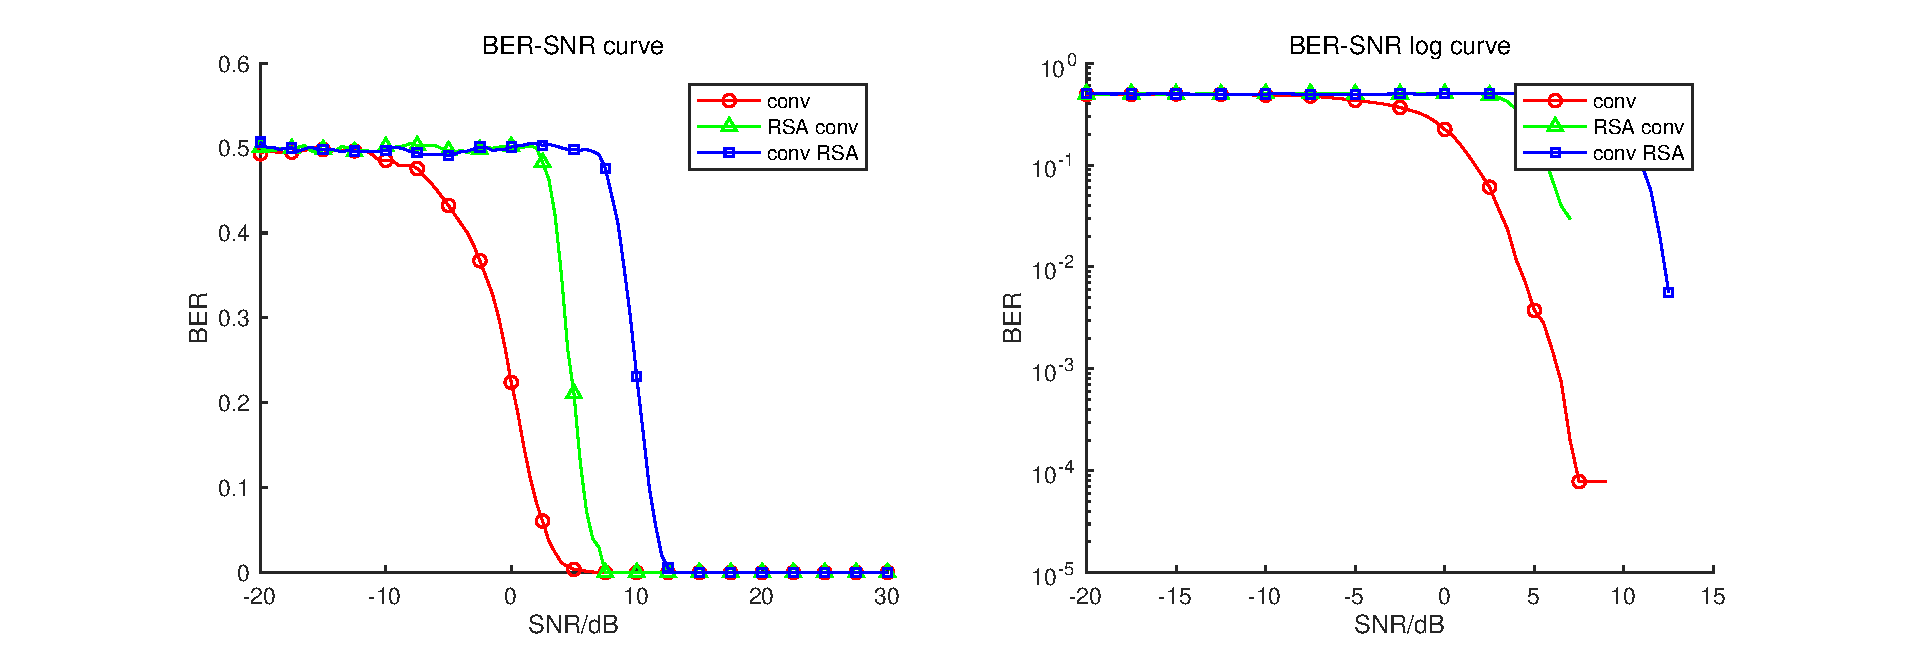
\includegraphics[width=6.0in]{./pic/rsamod0.eps}
	\caption{波形信道下的误码率曲线}
\end{figure}

\begin{figure}[h]
	\centering
    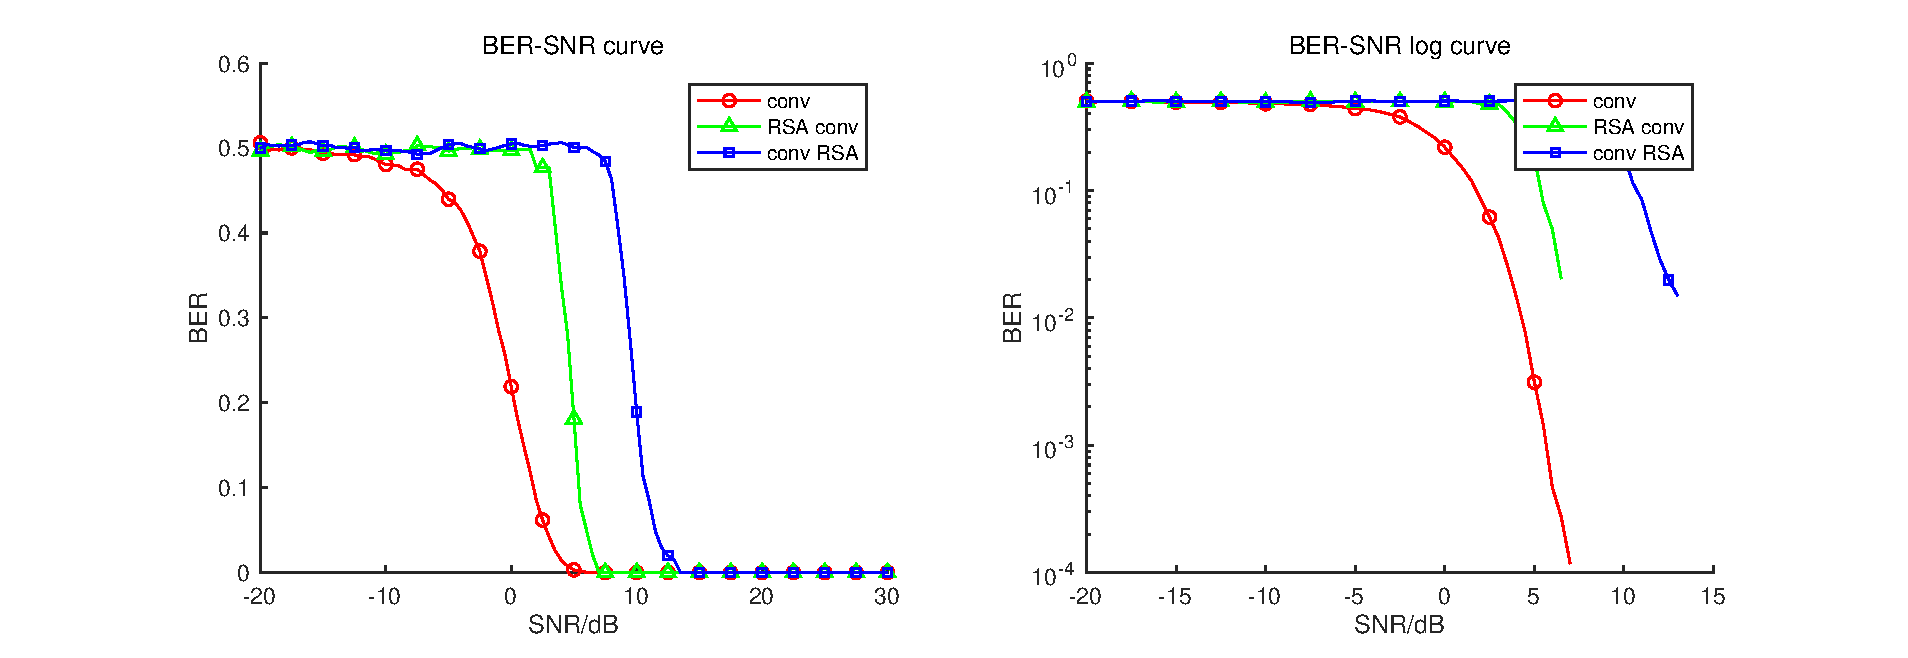
\includegraphics[width=6.0in]{./pic/rsamod1.eps}
	\caption{离散电平信道下的误码率曲线}
\end{figure}

\subsubsection{仿真分析}

AWGN波形信道和AWGN电平信道的误码率曲线的仿真结果几乎一样,因此我们不再区分他们,一起讨论。

\paragraph{结论1}RSA加密模块带来了明显的扩散效应。

相比于不加RSA模块,只有卷积模块的误码率曲线,RSA模块的加入让误码率曲线变得更加陡峭。体现了RSA模块带来的扩散效应-要么不错,要么几乎都错。所以才会让误码率曲线更加陡峭(要么是0.5的误码率,都错;要么是近乎0的误码率,不错)。

\paragraph{结论2}RSA加密模块加重了误码率。

两个加入了RSA加密模块的曲线无论在线性坐标下还是在对数坐标都向右偏移了,说明加密模块让通信变的更加不鲁棒,即更容易出错。这个结果是非常合理的,在密码的设计中,一个好的密码应该具有扩散性,即被攻击者修改了一点密文后,解密的明文应该会产生很大的变化。这样能够让接受者察觉到传输可能出现了问题。但是扩散性就会导致,如果密文因为信道的失真而产生了一些误bit,那么会导致难以恢复,并且在明文处产生更多的错误。因此通信的保密性需要建立在可靠性的基础上,我们通过提高通信的可靠性来换取一定的保密性。只有卷积码模块的时候,在大约SNR=7dB的时候,几乎没有误码率;而RSA+conv虽然在7dB之前的时候,性能比conv模块差,但是只有conv模块是在同一个SNR下无比特率为0的。因此,RSA+conv在良好的信噪比下(大于10dB)和conv模块相比是有相同性能的。

\paragraph{结论3}RSA加密模块应该在信道编码之前。

从仿真结果来看,RSA+conv的模块组合相比于只有conv模块有了一些性能上的下降;但是 conv+RSA相比于RSA+conv模块的性能有很大的下降。这是因为如果我们先进行信道编码,再进行加密的话,最外层的编码就是我们的加密算法,他的鲁棒性很差,有扩散效果,在经历了信道之后,有一点的错误就会扩散到的很严重,之后再进行信道编码的解码的时候就可以认为是经历了更低的信噪比下的一个信道,因此他的性能要RSA+conv差。

同时,由于如果先进行信道编码,再进行加密,那么我们加密的明文就是有冗余的明文,这样会让攻击者破解我们的加密变得更加容易,因此从这个角度来看,也应该先通过加密模块,再通过信道编码模块。

\subsection{误码图案}
\begin{figure}[h]
		\centering
		\subfigure[-10dB]{
			\includegraphics[width=1in]{./pic/pc1.eps}
		}
		\subfigure[-5dB]{
			\includegraphics[width=1in]{./pic/pc4.eps}
		}
		\subfigure[0dB]{
			\includegraphics[width=1in]{./pic/pc2.eps}
		}
		\subfigure[5dB]{
			\includegraphics[width=1in]{./pic/pc5.eps}
		}
		\subfigure[10dB]{
			\includegraphics[width=1in]{./pic/pc3.eps}
		}
		\caption{conv模式下各信噪比下典型误码图案}	
\end{figure}

\begin{figure}[h]
		\centering
		\subfigure[-10dB]{
			\includegraphics[width=1in]{./pic/pac1.eps}
		}
		\subfigure[-5dB]{
			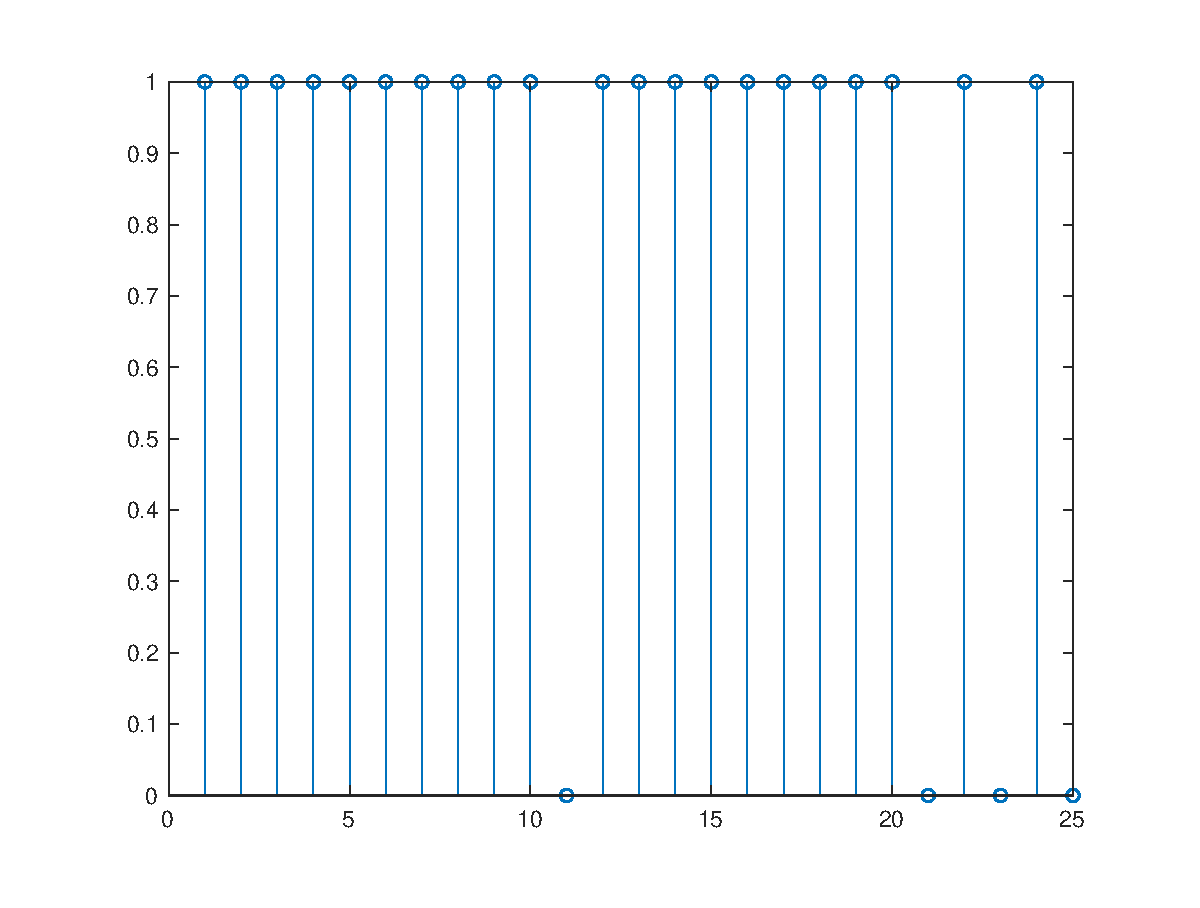
\includegraphics[width=1in]{./pic/pac4.eps}
		}
		\subfigure[0dB]{
			\includegraphics[width=1in]{./pic/pac2.eps}
		}
		\subfigure[5dB]{
			\includegraphics[width=1in]{./pic/pac5.eps}
		}
		\subfigure[10dB]{
			\includegraphics[width=1in]{./pic/pac3.eps}
		}
		\caption{RSA+conv模式下各信噪比下典型误码图案}	
\end{figure}

\begin{figure}[h]
		\centering
		\subfigure[-10dB]{
			\includegraphics[width=1in]{./pic/pca1.eps}
		}
		\subfigure[-5dB]{
			\includegraphics[width=1in]{./pic/pca4.eps}
		}
		\subfigure[0dB]{
			\includegraphics[width=1in]{./pic/pca2.eps}
		}
		\subfigure[5dB]{
			\includegraphics[width=1in]{./pic/pca5.eps}
		}
		\subfigure[10dB]{
			\includegraphics[width=1in]{./pic/pca3.eps}
		}
		\caption{conv+RSA模式下各信噪比下典型误码图案}	
\end{figure}

\paragraph{}由于卷积码是有记忆性的,因此他的错误是突发的。同时,加密模块由于有扩散效果,因此他的错误也是有突发的特点。因此我们能看到各个信噪比下的误码图案都是非常集中的。同时,由于误码率最高为0.5,因此有这种集中的错误,也就有一些对应的集中正确的图案。同时,由于在-10、-5两个信噪比下,三种方法的误码率都是0.5bit,因此误码图案上的错误非常密集。在0dB 的时候,conv方法的误码率已经下降,但是另外两种方法的误码率仍然为0.5,因此典型的误码图案的错误仍然很多。在5dB的时候,conv方法的误码率已经很低了,从图中也能看出来误码非常少了,同时另外两种方法的误码率也下降,误码图案中的误码也没有之前那么多了。在10dB的时候,三种方法都达到了0的误码率,误码图案也都是没有错误。


\section{椭圆加密}

\subsection{加密原理}

\subsubsection{$R^2$上的椭圆曲线}

我们把形如$y^2+axy+by=x^3+cx^2+dx+e$的三次方程称为椭圆曲线。我们通过在椭圆曲线上定义一个Abel群(可交换群),来完成在椭圆曲线上的算数运算。具体方法如下:

在椭圆曲线上任取两个点P、Q,其连线与椭圆曲线交于唯一点$T‘(t’_x,t‘_y)$。T'关于x轴的对称点$T(t_x,t_y)$是加法P和Q两点在椭圆曲线算数意义下的和,即P+Q=T。

如果Q=P,那么P和Q的连线就取为P点处椭圆曲线上的切线。

如果P、Q的连线和椭圆曲线没有其他的交点,那么我们就认为这条曲线和椭圆曲线相交于无穷远点。并且取无穷远点为椭圆曲线算数意义下的零元。

\begin{figure}[h]
	\centering
		\includegraphics[width=6.0in]{./pic/2_1.eps}
	\caption{$R^2$上的椭圆曲线$^{[1]}$}
\end{figure}

\subsubsection{GF(p)上的椭圆曲线}

在加密中,我们需要将椭圆曲线上点的取值限定在有限域。因此,我们定义GF(p)上的椭圆曲线。我们采用将变量和系数限制在集合$\{0,1,\cdot\cdot\cdot,p-1\}$上来进行模p运算。当将椭圆曲线限制在素域上时,我们将椭圆曲线限制为如下形式,
\begin{equation*}
y^2=x^3+ax+b\ mod\ p
\end{equation*}

并且将这个GF(p)上由系数a,b确定的椭圆曲线记为$E_p(a,b)$。并且将无穷远点记为O。

\begin{figure}[h]
	\centering
		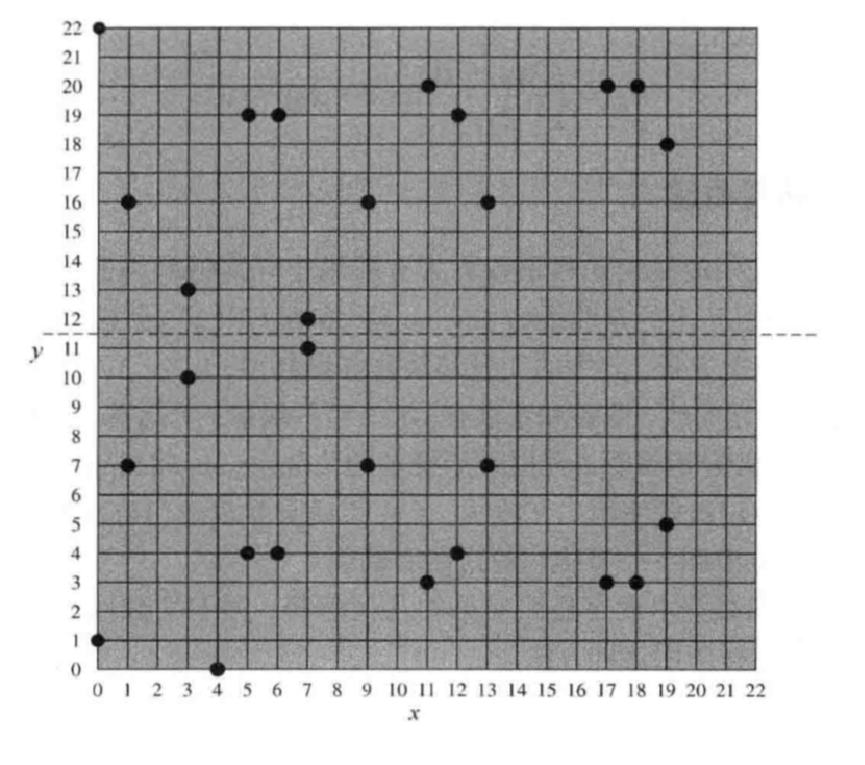
\includegraphics[width=0.5\textwidth]{./pic/2_2.eps}
	\caption{椭圆曲线$E_{23}$(1,1)$^{[1]}$}
\end{figure}

\paragraph{}椭圆曲线上的加密就是利用离散对数难解的特点,即给定P和T,并且有T=nP,对应的n的求解是很难的。

\subsubsection{GF(p)上的椭圆曲线加密}

首先,确定一个椭圆曲线$E_p(a,b)$,并且得到这个曲线上的生成元g。生成元的含义就是$kg\not=0\ s.t.\ k=0,1,2,\cdot\cdot\cdot, N-1$(N为$E_p(a,b)$上点的个数)。之后,随机生成一个大整数$x\ (x<p)$作为私钥匙,并且把$y=xg$作为公钥,并且把g和y公开。
\paragraph{}由于离散对数难解的特点,人们无法有效率的凭借g和y得到x的值,因此无法破解出私钥。并且这也是我们利用GF(p)上的椭圆曲线进行加密的基础。

\subsubsection{密钥交换}

GF(p)上的椭圆加密是非对称加密,相较于RSA,其更适合于进行密钥交换的任务,即双方在没有任何对称加密的情况下,传递加密的密钥。方法如下:

\begin{enumerate}
    \item Alice产生自己的私钥和公钥$x_a,y_a$;
    \item Bob产生自己的私钥和公钥$x_b,y_b$;
    \item Alice和Bob得到对方的公钥,并且Alice利用自己的私钥计算$T_a=x_ay_b=x_ax_bg$,Bob利用自己的私钥计算$T_b=x_by_a=x_ax_bg$;
    \item 显然有$T=T_a=T_b$,因此就可以根据双方约定的函数f,将T映射到双方约定的某一种对称加密的密钥key上,$key=f(T)$。
\end{enumerate}

\subsection{系数选取}

我们选取p和其对应的系数a、b以及生成原的时候,是参考文献Standards for Efficient Cryptography (SEC)$^[2]$中的一些成熟的标准进行的,并没有自己进行设计。p是我们选取的素数,a、b为椭圆曲线的系数,$g_x,g_y$为生成元g的坐标,n为g的阶。

下面是一组常用的112bit加密的ECC加密参数。

\begin{itemize}
    \item p=DB7C 2ABF62E3 5E668076 BEAD208B
    \item a=DB7C 2ABF62E3 5E668076 BEAD2088
    \item b=659E F8BA0439 16EEDE89 11702B22
    \item $g_x$=0948 7239995A 5EE76B55 F9C2F098
    \item $g_y$=A89C E5AF8724 C0A23E0E 0FF77500
    \item n=DB7C 2ABF62E3 5E7628DF AC6561C5
\end{itemize}

\subsection{整体流程}

我们要进行通信的双方,先随机生成各自的私钥x,再根据约定的椭圆曲线$E_p(a,b)$和生成元g产生各自的公钥。之后可以通过无加密的信道交换公钥,之后就能得到相同的交换密钥T。然后再根据双方约定的对称加密算法和交换密钥T到对称加密算法密钥的映射$f$,就能够得到对称加密所公用的密钥,并进行通信。

\begin{figure}[h]
	\centering
		\includegraphics[width=0.45\textwidth]{./pic/2_3.eps}
	\caption{密钥交换流程}
\end{figure}
